\documentclass[a4paper,12pt,oneside]{book}
\usepackage{lesi/lesi}
\usepackage[backend=biber, style=numeric, sorting=none]{biblatex}
\addbibresource{referencias.bib}
\usepackage{booktabs}
\usepackage{tabularx}
\usepackage{array}
\usepackage{longtable}
\usepackage{float}
\usepackage[table]{xcolor}
\usepackage{array}
\usepackage{ragged2e}
\usepackage{enumitem}
\usepackage{booktabs}
\usepackage{tabularx}
\usepackage{array}
\usepackage{longtable}
\usepackage{xcolor}
\newcolumntype{L}{>{\raggedright\arraybackslash}X}

\title{GrabATable}
\subtitle{Desenvolvimento de Interfaces Aplicacionais}
\author{Edgar Baptista, André Costa, João Ribeiro - Grupo 3}
\nrAluno{16447, 21087, 23795}
\regimePosLaboral
%\regimeDiurno          ou \regimePosLaboral
\LESI
\date{2026/2027}

%% Caso tenham mais que um orientador, colocar
%% \orientador{Nome professor \AND Nome professor}
\orientador{Marisa Pinheiro}

\dataEntrega{\textbf{Data de entrega:} 9 novembro - Entrega Final}

%% comentar estas três linhas para projectos
%\empresa{The Great Team}
%\enderecoEmpresa{Braga, Portugal}
%\supervisor{Eng. A. U. Thor}

% comentar se não for para usar glossários
%\makeglossaries



\begin{document}
\frontmatter
\maketitle  % print the title



%% Comment the following part if you are not acknowledging anybody
%\begin{agradecimentos}
%[A secção de agradecimentos é a parte pessoal do documento, e o único sítio onde o aluno pode escrever de forma menos formal, usando o tipo de linguagem que lhe parecer adequado para as pessoas a quem agradece.] 
%\end{agradecimentos}


\tableofcontents

% comentar se nao tiver figuraIs
\listoffigures

% comentar se nao tiver tabelas
\listoftables

% comentar se nao se quiser lista de codigo
%\lstlistoflistings

% Commentar proximas duas linhas se nao for para usar acronimos

% Commentar proximas duas linhas se nao for para usar glossarios
%\input{glossario}
%\printglossary

 
\mainmatter

\chapter{Introdução}

\section{Âmbito do Projeto}

\textbf{GrabATable – Plataforma de gestão de reservas de restaurantes}

A plataforma GrabATable consiste num sistema de gestão de reservas para restaurantes que combina dois mecanismos complementares: reservas antecipadas e gestão de fila de espera em tempo real para clientes sem reserva.

\subsection{Problema Identificado}

Os restaurantes que gerem reservas em papel, por telefone ou em sistemas isolados não conseguem conciliar as reservas com a afluência de clientes sem marcação. O resultado é sobrelotação, esperas imprevisíveis e uma má experiência tanto para quem reservou como para quem chegou sem reserva.

\subsection{Solução Proposta}

O cliente pode reservar mesa para uma data e hora, ou, ao chegar sem reserva, entrar numa fila virtual e acompanhar o tempo estimado. O sistema cruza reservas confirmadas, tempo médio de refeição e fila ativa para calcular a estimativa e avisa o
cliente quando a mesa estiver quase disponível. O sistema cruza continuamente a disponibilidade de mesas (reservas confirmadas, tempo médio de refeição e fila de espera atual) para calcular estimativas dinâmicas, notificando o cliente quando a mesa estiver próxima de ficar disponível.

\subsection{Inovação}

A fila de espera não é uma lista à parte: é um recurso gerido em conjunto com as
reservas, o que justifica uma arquitetura de microsserviços~\cite{newman,lewisfowler} (cálculo de espera a partir de
vários domínios, quase em tempo real).

\section{Público-Alvo e Tarefa Principal}

Há três perfis de utilizador, cada um com uma tarefa principal diferente.

\begin{table}[H]
    \centering
    \renewcommand{\arraystretch}{1.3}
    \begin{tabularx}{\textwidth}{@{}l X X X@{}}
        \toprule
        \textbf{Perfil} & \textbf{Quem é} & \textbf{Tarefa Principal} & \textbf{Contexto de uso} \\
        \midrule

        Cliente &
        Adultos dos 18 aos 55 anos, familiarizados com o uso do telemóvel &
        Reservar mesa ou entrar na fila e saber quanto tempo vai esperar &
        Telemóvel, muitas vezes a caminho do restaurante \\
        \midrule

        Gestor &
        Gerente ou responsável de sala de um restaurante &
        Gerir reservas, mesas e fila durante o serviço &
        Tablet ou computador, sob pressão de tempo \\
        \midrule

        Administrador &
        Equipa responsável pela plataforma &
        Configurar restaurantes, utilizadores e políticas globais &
        Computador, de forma pontual \\

        \bottomrule
    \end{tabularx}
    \caption{Público-alvo e tarefa principal}
    \label{tab:publico-alvo}
\end{table}

A tarefa central de todo o sistema é \textbf{garantir mesa sem surpresas:} o cliente sabe sempre se tem mesa e quando, e o gestor vê a ocupação e a fila num só ecrã.

\section{Objetivos}
O principal objetivo do projeto GrabATable é desenvolver uma plataforma de gestão de reservas e filas de espera para restaurantes, permitindo melhorar a organização da ocupação do estabelecimento e proporcionar aos clientes uma experiência mais previsível e eficiente.

A plataforma pretende centralizar a gestão de reservas antecipadas e de clientes sem reserva, utilizando a informação sobre a disponibilidade das mesas, reservas existentes, fila de espera e tempo médio de permanência para disponibilizar estimativas de espera atualizadas em tempo real.

Para concretizar o objetivo geral, o sistema deverá:
\begin{itemize}
    \item Permitir aos clientes consultar a disponibilidade de mesas e efetuar reservas para uma data e hora específicas;
    \item Permitir aos clientes entrar numa fila de espera virtual quando não possuem reserva;
    \item Disponibilizar ao cliente uma estimativa do tempo de espera, atualizada de acordo com a ocupação e rotatividade do restaurante;
    \item Notificar o cliente quando a sua mesa estiver próxima de ficar disponível;
    \item Permitir aos gestores dos restaurantes visualizar e gerir as reservas existentes;
    \item Permitir aos gestores gerir a fila de espera em tempo real;
    \item Permitir registar a chegada dos clientes, bem como situações de falta de comparência;
    \item Permitir aos gestores configurar e atualizar o estado das mesas do restaurante;
    \item Apoiar a distribuição dos clientes pelas mesas disponíveis de forma organizada;
    \item Permitir aos administradores gerir os restaurantes registados na plataforma;
    \item Permitir a configuração de políticas gerais da plataforma, como regras de falta de comparência e parâmetros relacionados com o tempo médio de refeição;
    \item Centralizar a informação relacionada com reservas, mesas e filas de espera numa única plataforma;
    \item Garantir uma interface simples e intuitiva, adequada aos diferentes perfis de utilizador;
    \item Melhorar a previsibilidade dos tempos de espera e reduzir situações de sobrelotação ou má gestão da capacidade do restaurante.
\end{itemize}

\section{Sistema Visual}\label{sec:sistema-visual}

A identidade combina um tom acolhedor, ligado à restauração, com interfaces limpas e legíveis.

\subsection{Logótipo}

\textit{Wordmark} "GrabATable" em tipografia arredondada, com o "A" no centro. O logótipo apresenta uma identidade visual moderna, minimalista e acolhedora, associada ao setor da restauração e à reserva de mesas em restaurantes. Combina um símbolo gráfico facilmente reconhecível com um nome de marca de grande destaque, utilizando uma paleta de cores que transmite frescura, confiança e proximidade.

\begin{figure}[H]
    \centering
    
\includegraphics[width=0.4\linewidth]{images/Logo.png}
    \caption{Logótipo}
    \label{fig:1}
\end{figure}

\subsection{Paleta Cromática}

A paleta cromática do GrabATable foi definida de forma a transmitir uma identidade visual simples, elegante e associada ao contexto de restauração.
A paleta cromática foi gerada com a ferramenta Coolors~\cite{coolors}.

\begin{figure}[H]
    \centering
    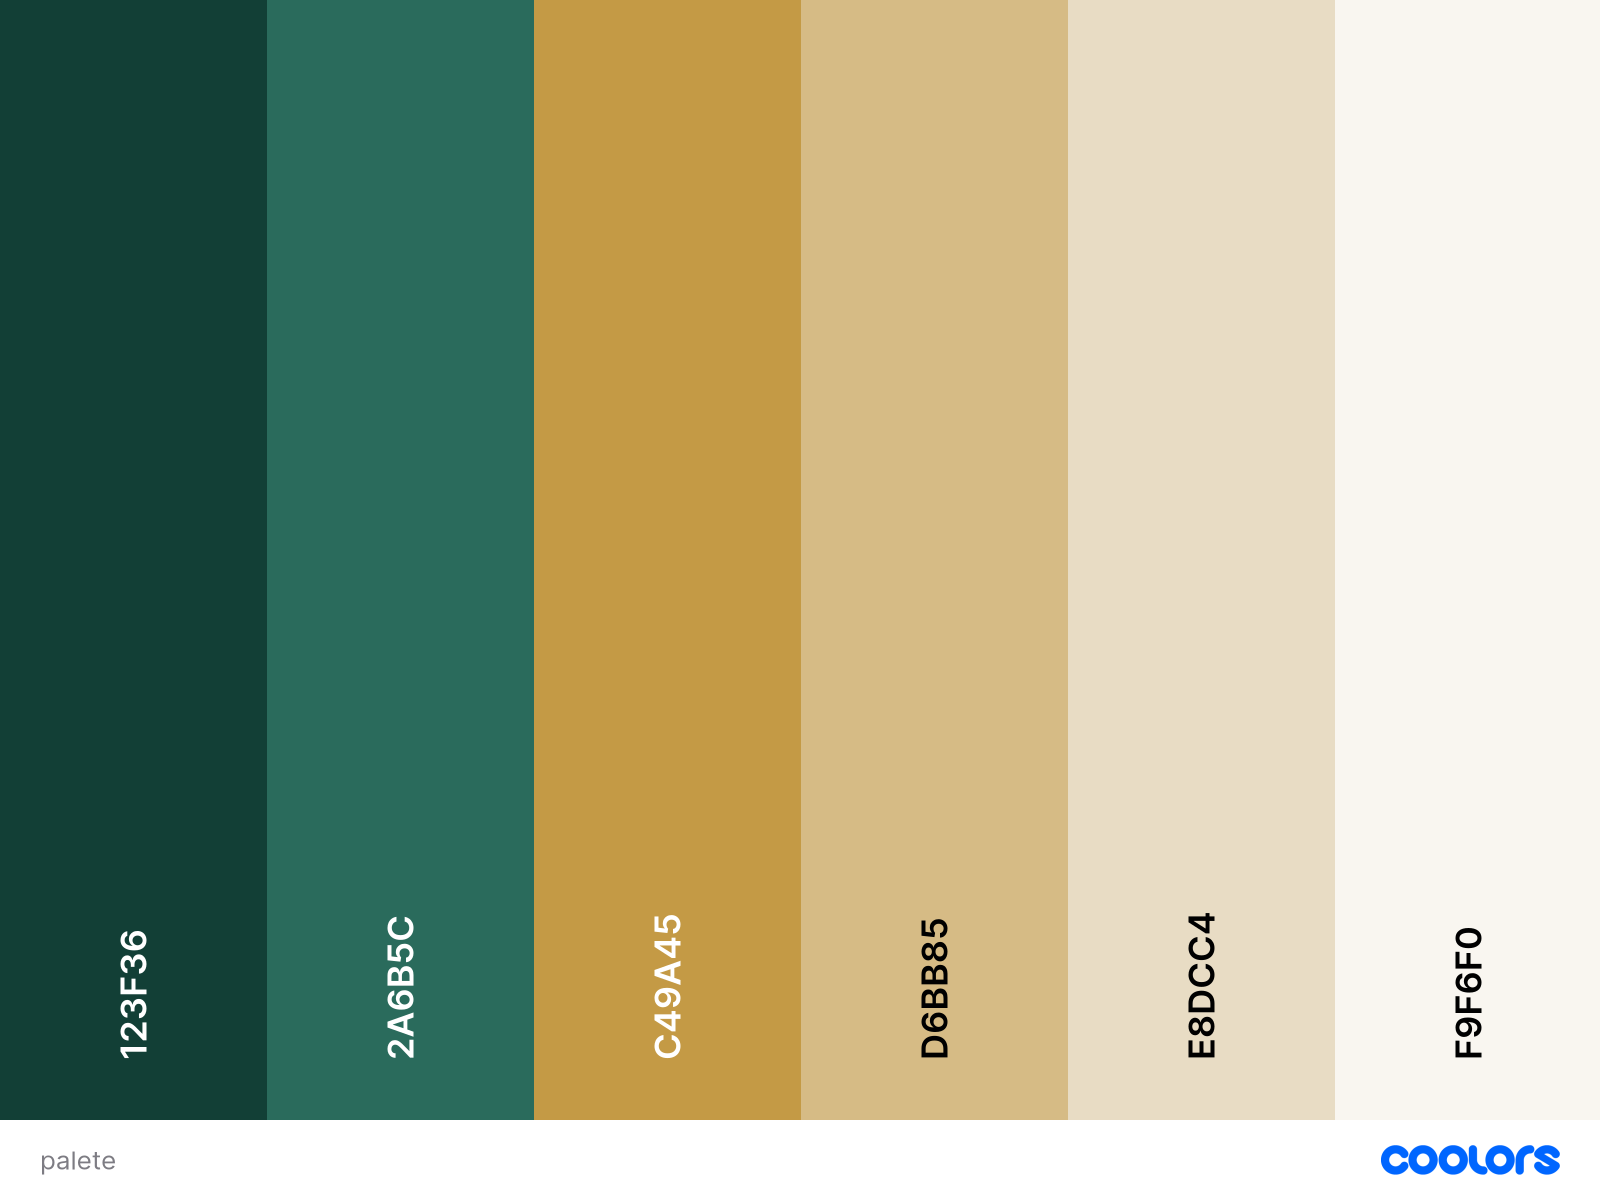
\includegraphics[width=0.6\linewidth]{images/paleta.png}
    \caption{Paleta Cromática}
    \label{fig:2}
\end{figure}

\begin{table}[H]
    \centering
    \renewcommand{\arraystretch}{1.3}
    \begin{tabularx}{\textwidth}{@{}l X X X@{}}
        \toprule
        \textbf{Papel} & \textbf{Nome} & \textbf{Hex} & \textbf{Uso} \\
        \midrule

        Primária &
        Verde floresta &
        \#123F36 &
        Texto principal, títulos, cabeçalhos \\
        \midrule

        Secundária &
        Verde &
        \#2A6B5C &
        Botões principais, ligações, estado confirmado \\
        \midrule

        Destaque &
        Ouro &
        \#C49A45 &
        Fila de espera, ícones e realces \\
        \midrule

        Apoio &
        Areia &
        \#D6BB85 &
        Etiquetas e fundos de realce, só com texto escuro \\
        \midrule

        Superfície &
        Bege &
        \#E8DCC4 &
        Cartões, separadores e campos \\
        \midrule

        Fundo &
        Creme &
        \#F9F6F0 &
        Fundo das páginas \\
        \midrule

        Erro &
        Vermelho &
        \#B91C1C &
        Erros e cancelamentos \\

        \bottomrule
    \end{tabularx}
    \caption{Paleta cromática}
    \label{tab:paleta-cromatica}
\end{table}

\subsection{Tipografia}

Títulos em \textit{Poppins} \textit{SemiBold} e texto corrido em Inter Regular, ambas gratuitas (Google \textit{Fonts}~\cite{googlefonts}). Escala: 32, 24, 20 px para títulos; 16 px para texto; 14 e 12 px para apoio. Altura de linha 1,5 no texto corrido.

\subsection{Grelha e Margens}

\subsubsection{Escala de espaçamento}

\begin{itemize}
    \item \textbf{4–8 px:} entre ícone e texto, ou dentro de componentes;
    \item \textbf{12–16 px:} \textit{padding} de botões e cartões, e espaço entre campos de formulário;
    \item \textbf{24–32 px:} entre grupos de conteúdo;
    \item \textbf{48–80 px:} entre secções da página.
\end{itemize}

\subsubsection{Grelha de colunas por tipo de dispositivo}

\begin{table}[H]
    \centering
    \renewcommand{\arraystretch}{1.1}
    \begin{tabularx}{\textwidth}{@{}l L L L L@{}}
        \toprule
        \textbf{Dispositivo} & \textbf{Largura do ecrã} & \textbf{Colunas} & \textbf{Margem lateral} & \textbf{\textit{Gutter} (Espaço entre colunas)} \\
        \midrule
        Telemóvel  & $<$ 600 px     & 4  & 16 px         & 16 px \\
        \midrule
        Tablet     & 600-839 px    & 8  & 24 px         & 24 px \\
        \midrule
        Computador & $\geq$ 1200 px & 12 & 32 px ou mais & 24--32 px \\
        \bottomrule
    \end{tabularx}
    \caption{Grelha responsiva por tipo de dispositivo}
    \label{tab:grelha}
\end{table}



\subsection{Componentes Principais}

\begin{itemize}
    \item Botão primário, secundário e de texto, com estados normal, foco, premido e desativado;
    \item Cartão de restaurante (foto, nome, cozinha, disponibilidade);
    \item Seletor de data, hora e número de pessoas;
    \item Indicador de tempo de espera, com minutos e posição na fila;
    \item Etiqueta de estado da reserva (pendente, confirmada, cancelada, não comparência);
    \item Barra de navegação por perfil e menu lateral de gestão;
    \item Tabela de gestão com filtros e ações por linha;
    \item Notificações e alertas de erro em formulários.
\end{itemize}

\subsection{Acessibilidade Cromática}

O texto escuro sobre fundos claros e o texto claro sobre verde passam o nível AA da \textit{WCAG} 2.1~\cite{wcag} (mínimo 4,5:1 para texto normal); o ouro e a areia falham com texto claro ou verde. Os rácios foram calculados com a fórmula de luminância relativa da \textit{WCAG}.

\begin{table}[H]
    \centering
    \renewcommand{\arraystretch}{1.3}
    \begin{tabularx}{\textwidth}{@{}l X X@{}}
        \toprule
        \textbf{Texto / fundo} & \textbf{Rácio} & \textbf{AA (4,5:1)} \\
        \midrule

        Verde floresta / Creme &
        10,88 &
        Passa \\
        \midrule

        Verde floresta / Bege &
        8,64 &
        Passa \\
        \midrule

        Verde floresta / Areia &
        6,32 &
        Passa \\
        \midrule

        Vermelho / Creme &
        6,00 &
        Passa \\
        \midrule

        Verde / Creme &
        5,80 &
        Passa \\
        \midrule

        Verde / Bege &
        4,61 &
        Passa \\
        \midrule

        Verde floresta / Ouro &
        4,50 &
        Passa, por margem mínima \\
        \midrule

        Verde / Areia &
        3,37 &
        Falha \\
        \midrule

        Branco / Ouro &
        2,61 &
        Falha \\
        \midrule

        Creme / Ouro &
        2,42 &
        Falha \\
        \midrule

        Verde / Ouro &
        2,40 &
        Falha \\
        \midrule

        Ouro / Bege &
        1,92 &
        Falha \\

        \bottomrule
    \end{tabularx}
    \caption{Acessibilidade cromática}
    \label{tab:acessibilidade-cromatica}
\end{table}

\subsubsection{Problema encontrado}

A legenda do diagrama usa texto branco sobre amarelo (1,84), verde (2,28) e vermelho (3,76), e todas falham. Correção: texto Carvão
sobre o amarelo (7,98) e sobre o verde, ou substituir os círculos por etiquetas com texto.

\subsubsection{Regras adotadas}

\begin{itemize}
    \item O ouro nunca leva texto claro nem verde por cima; com ele usa-se Verde floresta (4,50:1, no limite);
    \item Ouro sobre Creme dá 2,42:1, abaixo dos 3:1 exigidos a ícones e bordas, pelo que estes usam Verde (5,80:1) e o ouro fica só como realce;
    \item A cor nunca é o único meio de informação: estados de reserva e fila têm sempre texto e ícone;
    \item Foco de teclado visível, com contorno de 2 px em Verde.
\end{itemize}
\chapter{Análise e Modelação do Sistema}

\section{Site Map}

O Site Map apresenta a estrutura e organização das principais páginas que constituem o sistema GrabATable, permitindo visualizar a hierarquia de navegação e a forma como as diferentes áreas e funcionalidades se encontram interligadas. Este permite também identificar os diferentes perfis de utilizador e as páginas e funcionalidades a que cada perfil terá acesso, proporcionando uma visão global da estrutura e navegação da plataforma.

\begin{figure}[H]
    \centering
    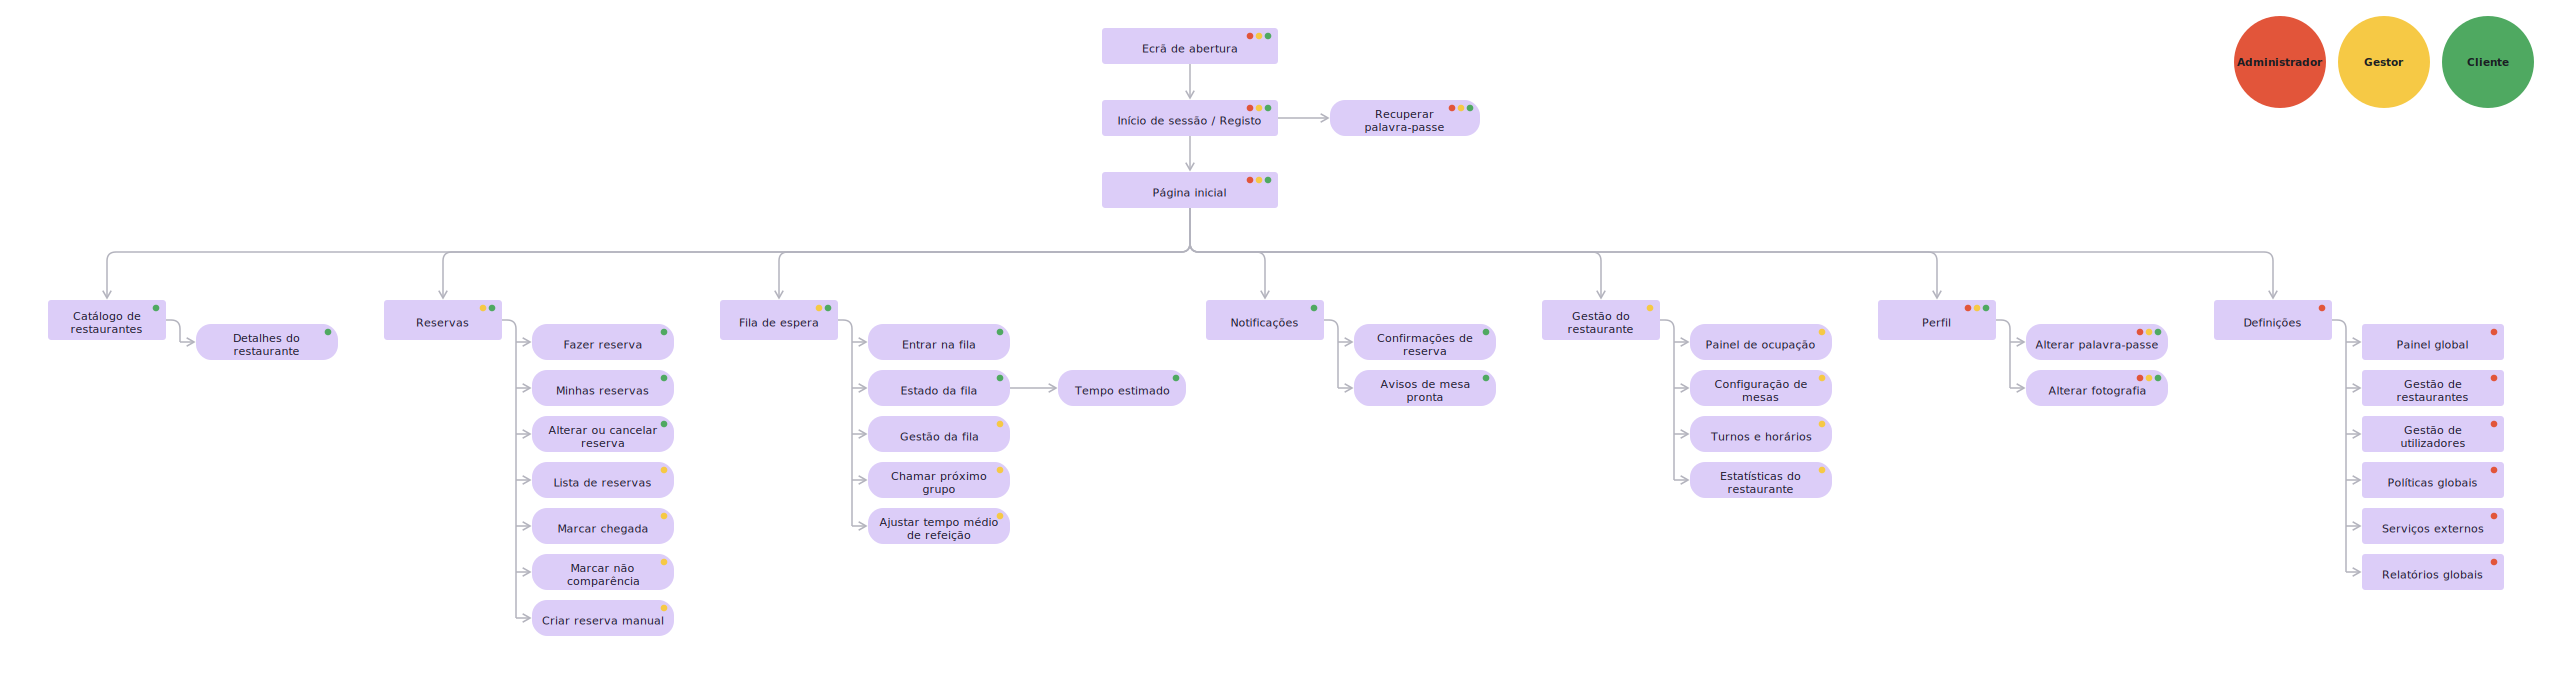
\includegraphics[width=1.0\linewidth]{images/Site_Map.png}
    \caption{Site Map}
    \label{fig:3}
\end{figure}

Todos os perfis partilham o ecrã de abertura, o registo e a página inicial.

\section{Task Model}\label{sec:task-model}

O \textit{Task Model} representa as principais tarefas que podem ser realizadas pelos diferentes perfis de utilizador no sistema GrabATable. Este modelo permite identificar e organizar as ações necessárias para a execução das principais funcionalidades da plataforma, evidenciando a relação entre os utilizadores e as tarefas que estes podem realizar.

\subsection{\textit{Task Model} - Administrador} 

\begin{figure}[H]
    \centering
    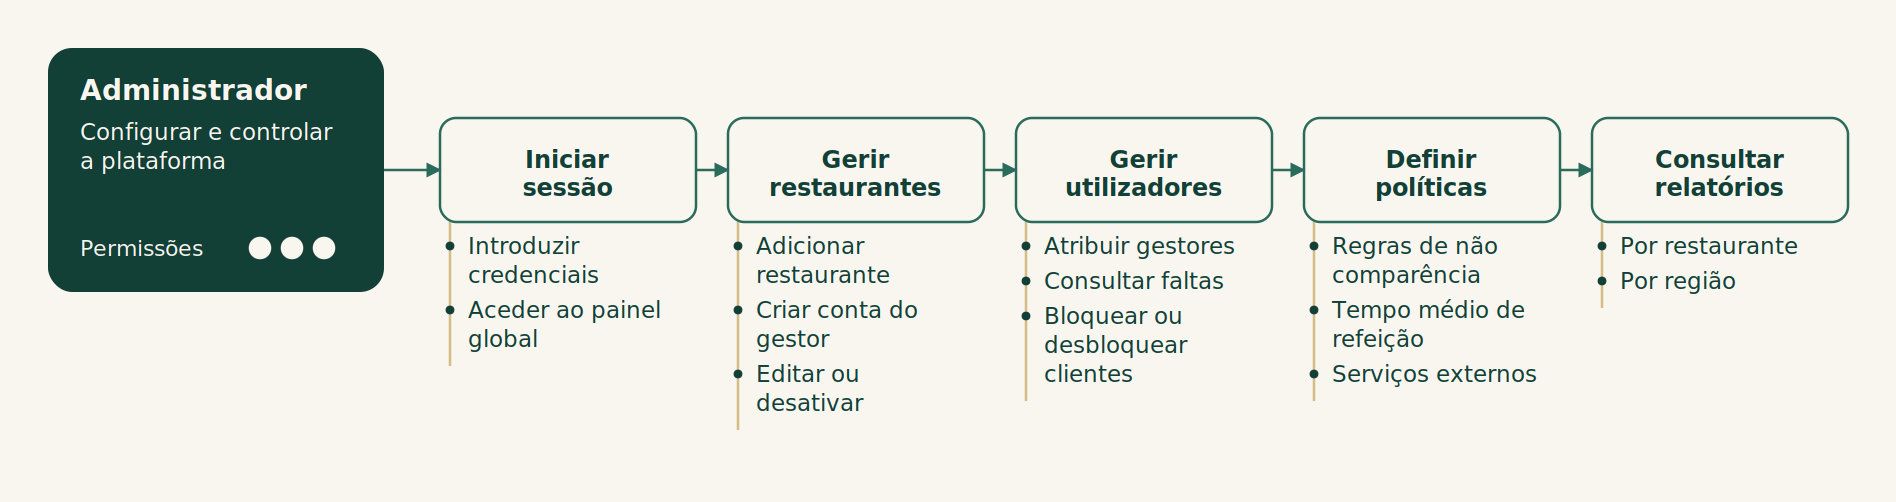
\includegraphics[width=1.0\linewidth]{images/Task_Model_Administrador.png}
    \caption{Task Model - Administrador}
    \label{fig:4}
\end{figure}

\subsubsection{Tarefa principal - Administrador}

Processo para um administrador adicionar um restaurante à plataforma.

\begin{figure}[H]
    \centering
    
\includegraphics[width=1.0\linewidth]{images/Task_Model_1_Administrador_horizontal.png}
    \caption{Tarefa principal - Administrador}
    \label{fig:5}
\end{figure}

\subsection{\textit{Task Model} - Gestor}

\begin{figure}[H]
    \centering
    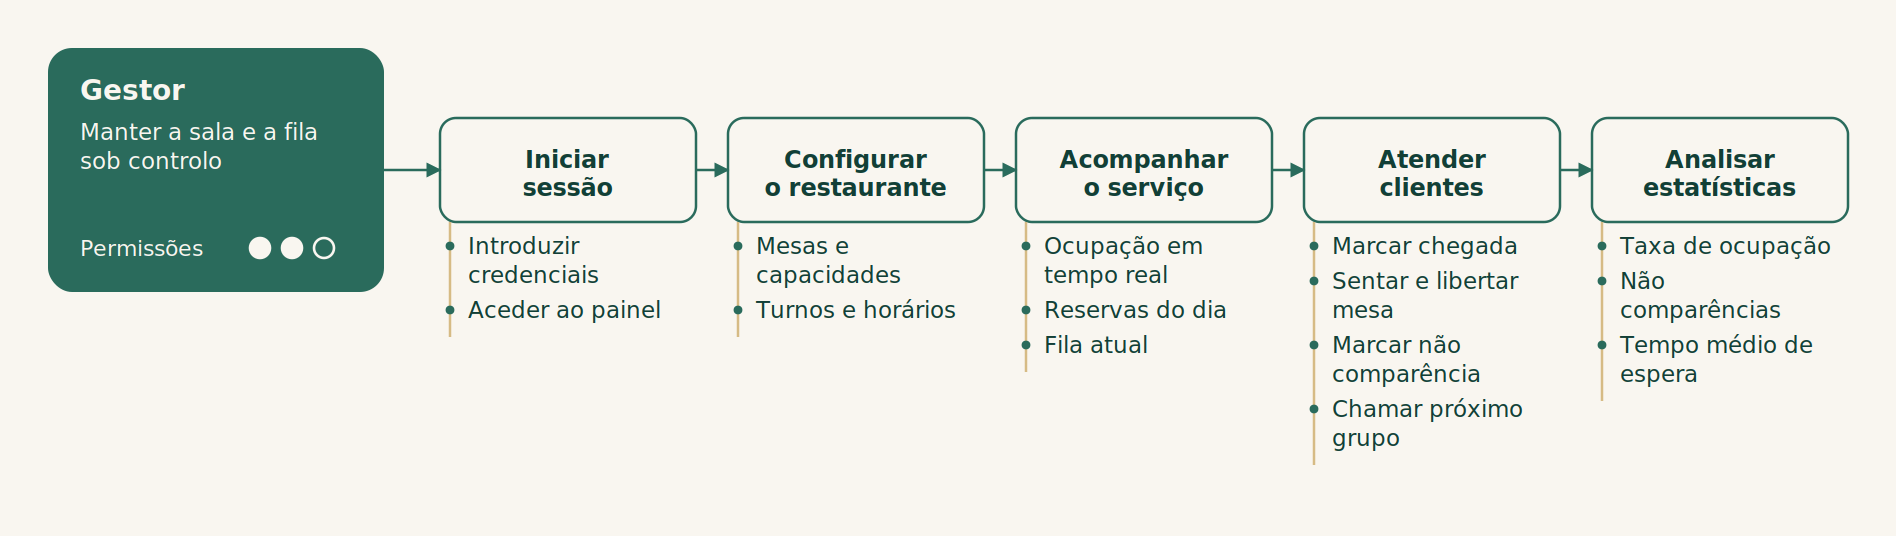
\includegraphics[width=1.0\linewidth]{images/Task_Model_Gestor.png}
    \caption{Task Model - Gestor}
    \label{fig:6}
\end{figure}

\subsubsection{Tarefa principal - Gestor}

Processo para um gestor atender um cliente com reserva.

\begin{figure}[H]
    \centering
    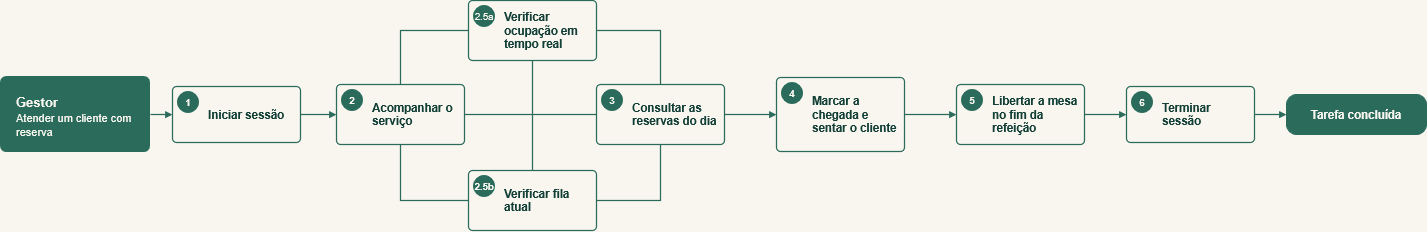
\includegraphics[width=1.0\linewidth]{images/Task_Model_2_Gestor_horizontal.png}
    \caption{Tarefa principal - Gestor}
    \label{fig:7}
\end{figure}

\subsection{\textit{Task Model} - Cliente}

\begin{figure}[H]
    \centering
    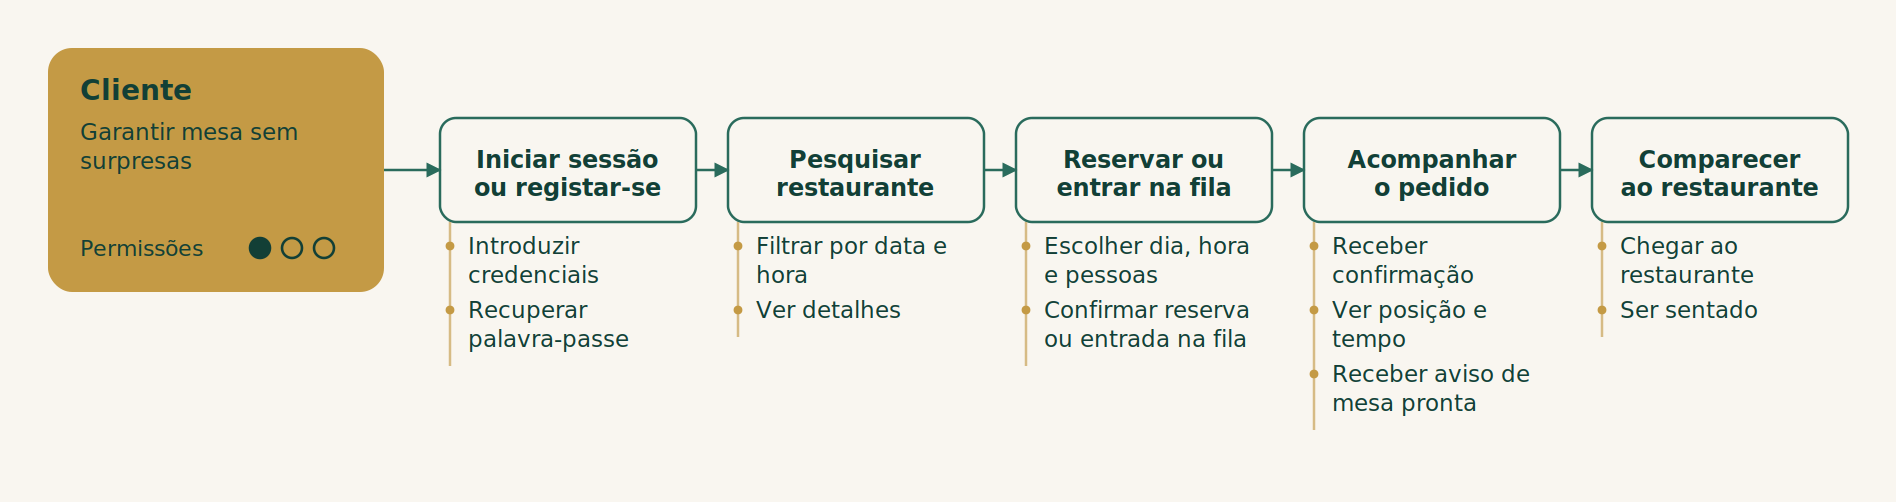
\includegraphics[width=1.0\linewidth]{images/Task_Model_Cliente.png}
    \caption{Task Model - Cliente}
    \label{fig:8}
\end{figure}

\subsubsection{Tarefa principal - Cliente}

Processo para um cliente reservar mesa para refeição.

\begin{figure}[H]
    \centering
    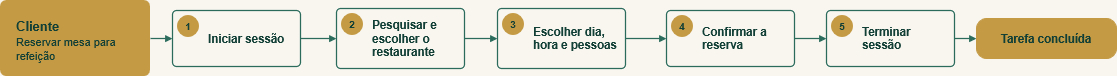
\includegraphics[width=1.0\linewidth]{images/Task_Model_3_Cliente_horizontal.png}
    \caption{Tarefa principal - Cliente}
    \label{fig:9}
\end{figure}

\section{Requisitos Funcionais e Não Funcionais}

Nesta secção são apresentados os requisitos do sistema GrabATable, definidos a partir das funcionalidades e necessidades identificadas para a plataforma. Os requisitos encontram-se divididos em requisitos funcionais, que descrevem as funcionalidades e comportamentos que o sistema deve disponibilizar, e requisitos não funcionais, que especificam características relacionadas com a qualidade, desempenho, segurança, usabilidade do sistema, entre outros.

\subsection{Requisitos Funcionais}
\label{chap:rf}

O sistema GrabATable possui 17 requisitos funcionais, agrupados de acordo com os diferentes perfis de utilizador da plataforma.

\begin{itemize}
    \setlength{\itemsep}{10pt}

    \item \textbf{RF01:} O sistema deve permitir que os utilizadores registem uma conta e iniciem sessão. \textbf{Prioridade:} Alta.

    \item \textbf{RF02:} O sistema deve permitir que os utilizadores recuperem a sua palavra-passe. \textbf{Prioridade:} Média.

    \item \textbf{RF03:} Os clientes devem poder pesquisar restaurantes por localização, tipo de cozinha, data e hora. \textbf{Prioridade:} Alta.

    \item \textbf{RF04:} Os clientes devem poder consultar os detalhes e a disponibilidade de um restaurante. \textbf{Prioridade:} Alta.

    \item \textbf{RF05:} Os clientes devem poder criar uma reserva indicando a data, hora e número de pessoas. \textbf{Prioridade:} Alta.

    \item \textbf{RF06:} Os clientes devem poder consultar, alterar e cancelar as suas reservas. \textbf{Prioridade:} Alta.

    \item \textbf{RF07:} Os clientes devem poder entrar na fila de espera e consultar a sua posição e o tempo estimado de espera. \textbf{Prioridade:} Alta.

    \item \textbf{RF08:} O sistema deve permitir que os clientes recebam notificações relativas à confirmação de uma reserva e à disponibilidade da mesa. \textbf{Prioridade:} Alta.

    \item \textbf{RF09:} Os gestores devem poder gerir as reservas do restaurante e registar a chegada ou não comparência dos clientes. \textbf{Prioridade:} Alta.

    \item \textbf{RF10:} Os gestores devem poder gerir a fila de espera, consultar a ordem dos clientes e chamar o próximo grupo. \textbf{Prioridade:} Alta.

    \item \textbf{RF11:} Os gestores devem poder configurar as mesas, respetivas capacidades, turnos e horários de funcionamento do restaurante. \textbf{Prioridade:} Alta.

    \item \textbf{RF12:} Os gestores devem poder consultar estatísticas relacionadas com a ocupação, não comparência e tempos de espera. \textbf{Prioridade:} Média.

    \item \textbf{RF13:} Os administradores devem poder criar, editar e remover restaurantes da plataforma. \textbf{Prioridade:} Alta.

    \item \textbf{RF14:} Os administradores devem poder gerir os utilizadores e bloquear clientes com um número excessivo de não comparências. \textbf{Prioridade:} Média.

    \item \textbf{RF15:} Os administradores devem poder definir políticas globais da plataforma, incluindo regras de não comparência e tempo médio de refeição. \textbf{Prioridade:} Média.

    \item \textbf{RF16:} Os administradores devem poder consultar relatórios globais organizados por restaurante e região. \textbf{Prioridade:} Baixa.

    \item \textbf{RF17:} O sistema deve permitir que os utilizadores alterem a sua palavra-passe e fotografia de perfil. \textbf{Prioridade:} Baixa.

\end{itemize}


\subsection{Requisitos Não Funcionais}
\label{chap:rnf}

O sistema GrabATable possui 9 requisitos não funcionais, relacionados com características de qualidade e restrições técnicas da plataforma.

\begin{itemize}
    \setlength{\itemsep}{10pt}

    \item \textbf{RNF01 -- Desempenho:} As consultas devem apresentar uma resposta inferior a 500 ms no percentil 95. A estimativa de espera deve ser atualizada em menos de 5 segundos após uma alteração.

    \item \textbf{RNF02 -- Segurança:} A autenticação deve utilizar \textit{JWT}, validado no API \textit{Gateway}, com comunicação através de HTTPS, palavras-passe armazenadas através de \textit{hash} e controlo de acesso por perfil.

    \item \textbf{RNF03 -- Segurança entre serviços:} Os microsserviços não devem ficar diretamente expostos a pedidos externos, sendo o API Gateway o único componente responsável pela receção de pedidos externos.

    \item \textbf{RNF04 -- Resiliência:} Uma falha no serviço de Notificações não deve impedir a criação de reservas, sendo utilizadas mensagens assíncronas para a comunicação entre serviços (RabbitMQ~\cite{rabbitmq}).

    \item \textbf{RNF05 -- Escalabilidade:} Os serviços devem ser \textit{stateless}, executados em \textit{containers} e preparados para escalabilidade horizontal através de \textit{Kubernetes}.

    \item \textbf{RNF06 -- Facilidade de Manutenção:} A arquitetura deve utilizar um microsserviço por área de negócio, com base de dados própria, migrações por versões e \textit{APIs} documentadas através de \textit{OpenAPI}.

    \item \textbf{RNF07 -- Usabilidade e acessibilidade:} A plataforma deve seguir uma abordagem \textit{mobile first} e permitir a realização das ações principais em, no máximo, três toques.

    \item \textbf{RNF08 -- Testabilidade:} Cada serviço deve possuir testes unitários, testes de integração e uma \textit{collection} Postman para validação das respetivas \textit{API's}.

    \item \textbf{RNF09 -- Privacidade:} A plataforma deve cumprir o \textit{RGPD}, garantindo a utilização mínima de dados, a obtenção de consentimento quando aplicável e a possibilidade de eliminação da conta.

\end{itemize}

\section{Arquitetura Técnica do Sistema}

A arquitetura técnica do sistema apresenta a organização dos principais componentes tecnológicos que constituem a plataforma GrabATable e a forma como estes comunicam entre si. Esta representação permite compreender a distribuição das diferentes camadas do sistema.

\begin{figure}[H]
    \centering
    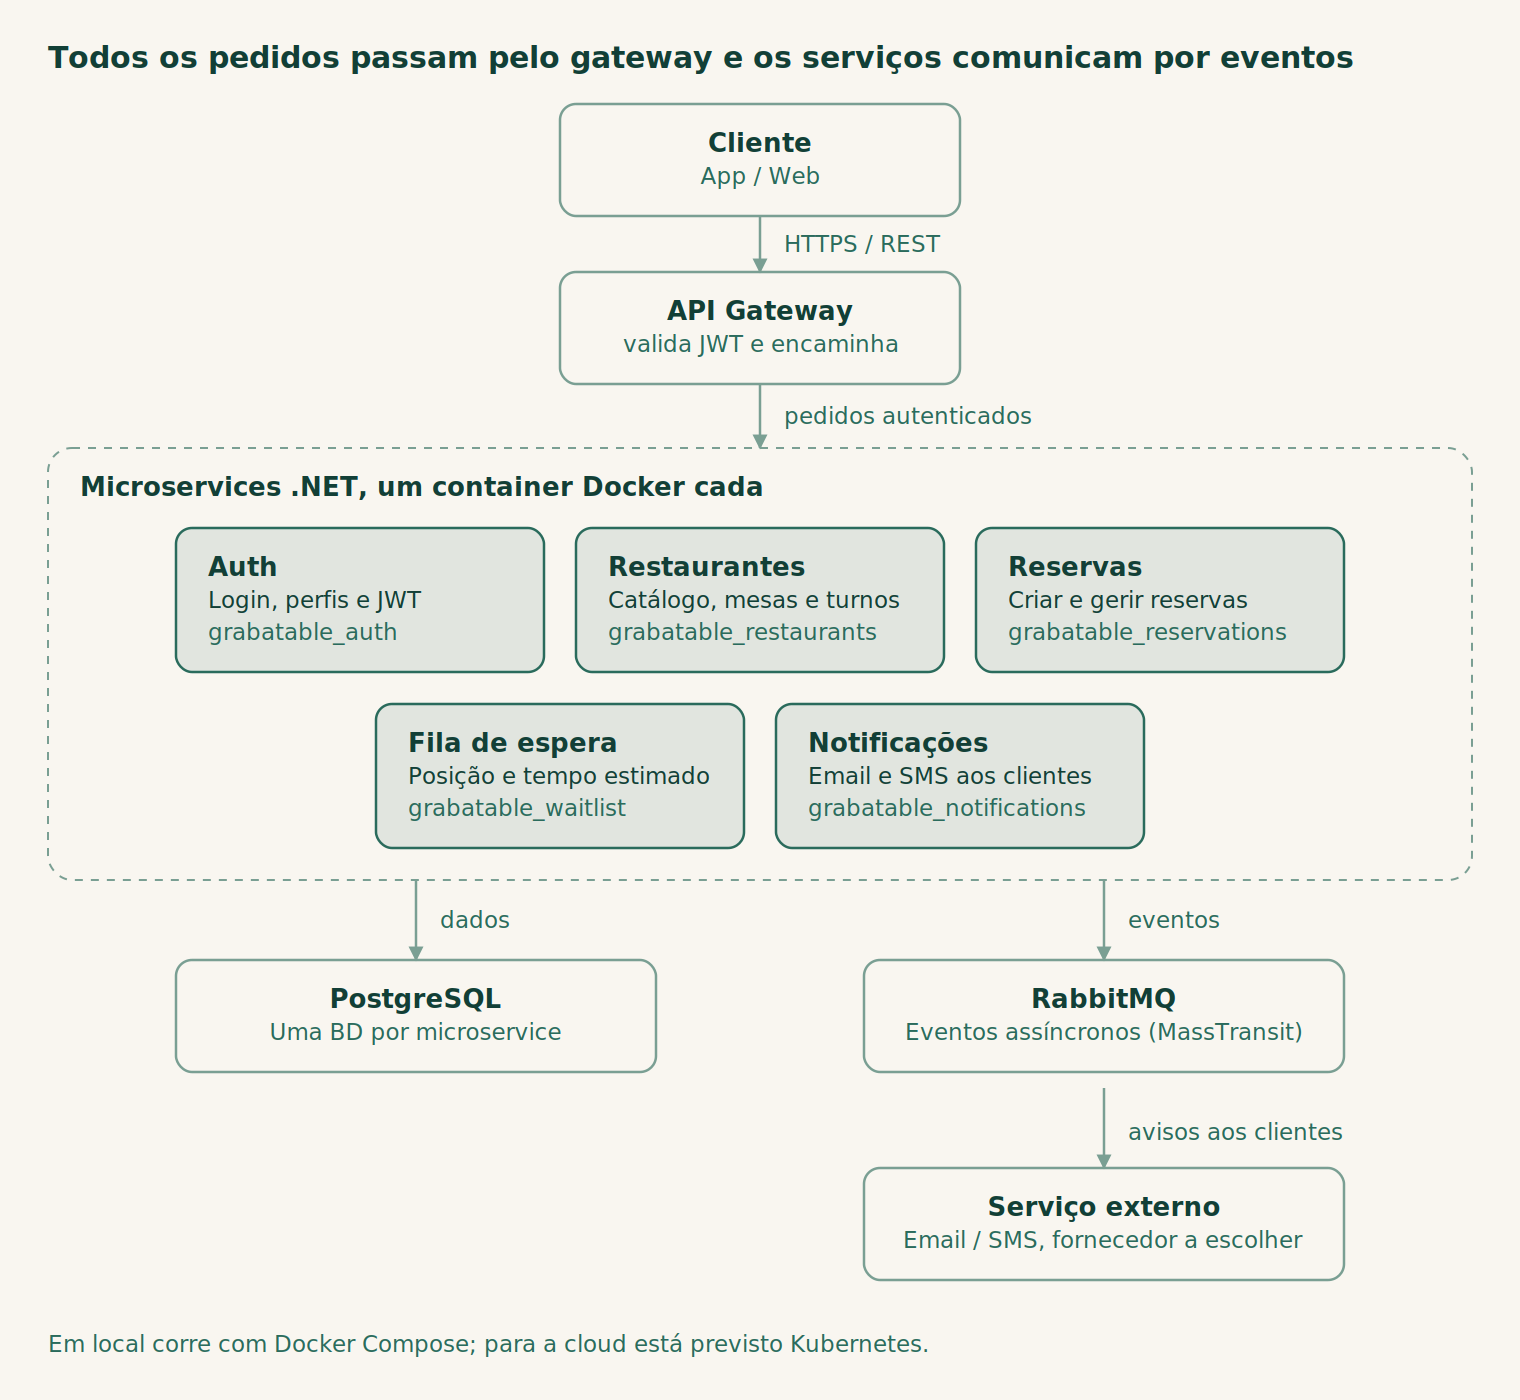
\includegraphics[width=1.0\linewidth]{images/arquitetura.png}
    \caption{Arquitetura Técnica do Sistema}
    \label{fig:10}
\end{figure}

O \textit{gateway} é o único ponto exposto: valida o \textit{JWT} e encaminha cada pedido para o microsserviço certo. Cada serviço tem a sua base de dados no mesmo PostgreSQL. Reservas e Fila de espera publicam eventos no \textit{RabbitMQ}~\cite{rabbitmq}, e o serviço de Notificações consome-os para avisar o cliente.

\section{BPMN}

O diagrama BPMN representa o fluxo dos principais processos do sistema GrabATable, permitindo visualizar de forma estruturada as atividades realizadas pelos diferentes intervenientes. Através deste modelo, é possível compreender a sequência das tarefas, as decisões e interações entre os diferentes participantes, proporcionando uma visão global do funcionamento dos processos da plataforma.

\begin{figure}[H]
    \centering
    
\includegraphics[width=1.0\linewidth]{images/BPMN.png}
    \caption{Diagrama BPMN}
    \label{fig:11}
\end{figure}

\section{Personas}
 
As \textit{personas} são perfis fictícios, construídos a partir dos três perfis de utilizador definidos na Secção 1.2, que representam os objetivos, o contexto de uso e as frustrações dos utilizadores reais da plataforma.
 
\subsection{Persona 1 -- Marta Silva (Cliente)}
 
\begin{tabularx}{\textwidth}{@{}>{\bfseries}p{3.4cm}X@{}}
\toprule
Perfil & Cliente \\
Idade e profissão & 34 anos, designer gráfica \\
Localização & Braga \\
Competência digital & Alta; usa o telemóvel para quase tudo, incluindo pagamentos e marcações \\
Contexto de uso & Telemóvel, em casa ou no trabalho, a organizar jantares com antecedência \\
\midrule
Objetivos &
\begin{itemize}[nosep,leftmargin=*]
  \item Reservar mesa para um grupo de 4 a 6 pessoas, sem telefonar;
  \item Ter confirmação imediata e poder alterar ou cancelar a reserva;
  \item Receber um lembrete antes da data.
\end{itemize} \\
Frustrações &
\begin{itemize}[nosep,leftmargin=*]
  \item Restaurantes que só aceitam reservas por telefone, em horário de expediente;
  \item Chegar à hora marcada e esperar por uma mesa que devia estar livre;
  \item Não saber se a reserva ficou realmente registada.
\end{itemize} \\
Cenário &
A Marta quer jantar com amigos na sexta-feira. Pesquisa restaurantes por cozinha e hora, confirma a disponibilidade para seis pessoas, reserva em poucos toques e recebe a notificação de confirmação. \\
Requisitos associados & RF03, RF04, RF05, RF06, RF08 \\
\bottomrule
\end{tabularx}
 
\subsection{Persona 2 -- Rui Fernandes (Cliente sem reserva)}
 
\begin{tabularx}{\textwidth}{@{}>{\bfseries}p{3.4cm}X@{}}
\toprule
Perfil & Cliente \\
Idade e profissão & 27 anos, técnico de logística \\
Localização & Guimarães \\
Competência digital & Média-alta; usa aplicações móveis no dia a dia, mas pouco paciente com processos longos \\
Contexto de uso & Telemóvel, muitas vezes a caminho do restaurante, com pouco tempo e uma só mão livre \\
\midrule
Objetivos &
\begin{itemize}[nosep,leftmargin=*]
  \item Entrar na fila antes de chegar ao restaurante;
  \item Saber a posição e o tempo estimado de espera;
  \item Ser avisado quando a mesa estiver quase pronta, para poder fazer outra coisa entretanto.
\end{itemize} \\
Frustrações &
\begin{itemize}[nosep,leftmargin=*]
  \item Esperas de pé, sem qualquer estimativa;
  \item Estimativas dadas ao balcão que nunca se cumprem;
  \item Perder a vez por ter saído para ir buscar o carro.
\end{itemize} \\
Cenário &
O Rui decide jantar fora de improviso. Abre a aplicação, escolhe um restaurante, entra na fila para duas pessoas e vê que a espera é de cerca de 25 minutos. Recebe um aviso quando a mesa está próxima de ficar disponível. \\
Requisitos associados & RF03, RF04, RF07, RF08 \\
\bottomrule
\end{tabularx}
 
\subsection{Persona 3 -- Teresa Almeida (Gestora)}
 
\begin{tabularx}{\textwidth}{@{}>{\bfseries}p{3.4cm}X@{}}
\toprule
Perfil & Gestor \\
Idade e profissão & 45 anos, responsável de sala num restaurante com 18 mesas \\
Localização & Porto \\
Competência digital & Média; usa tablet e computador, mas valoriza ferramentas simples \\
Contexto de uso & Tablet à entrada da sala, durante o serviço, sob pressão de tempo e com interrupções constantes \\
\midrule
Objetivos &
\begin{itemize}[nosep,leftmargin=*]
  \item Ver num só ecrã a ocupação das mesas, as reservas do dia e a fila;
  \item Registar chegadas, sentar clientes e libertar mesas com poucos toques;
  \item Reduzir as faltas de comparação e a sobrelotação.
\end{itemize} \\
Frustrações &
\begin{itemize}[nosep,leftmargin=*]
  \item Caderno de reservas em papel e lista de espera improvisada;
  \item Mesas reservadas que ficam vazias por não comparência;
  \item Clientes sem reserva que se queixam de esperas sem explicação.
\end{itemize} \\
Cenário &
Em plena hora de ponta, a Teresa regista a chegada de um grupo com reserva, vê que há uma mesa a libertar-se e chama o próximo grupo da fila, sem sair do tablet. \\
Requisitos associados & RF09, RF10, RF11, RF12 \\
\bottomrule
\end{tabularx}
 
\subsection{Persona 4 -- Pedro Machado (Administrador)}
 
\begin{tabularx}{\textwidth}{@{}>{\bfseries}p{3.4cm}X@{}}
\toprule
Perfil & Administrador \\
Idade e profissão & 38 anos, membro da equipa responsável pela plataforma \\
Localização & Remoto \\
Competência digital & Muito alta; confortável com painéis de administração e relatórios \\
Contexto de uso & Computador, de forma pontual, para configurar e supervisionar \\
\midrule
Objetivos &
\begin{itemize}[nosep,leftmargin=*]
  \item Adicionar e configurar novos restaurantes e respetivas contas de gestor;
  \item Definir políticas globais (regras de não comparência, tempo médio de refeição);
  \item Consultar relatórios por restaurante e por região.
\end{itemize} \\
Frustrações &
\begin{itemize}[nosep,leftmargin=*]
  \item Configurações dispersas por vários ecrãs;
  \item Falta de histórico sobre quem alterou o quê;
  \item Dificuldade em identificar clientes com faltas repetidas.
\end{itemize} \\
Cenário &
O Pedro integra um novo restaurante: cria o registo, cria a conta do gestor e confirma a configuração, tudo a partir da Gestão de restaurantes. \\
Requisitos associados & RF13, RF14, RF15, RF16 \\
\bottomrule
\end{tabularx}
 
 
% ============================================================
 
\section{Análise SWOT}
 
A análise SWOT identifica os fatores internos (forças e fraquezas) e externos (oportunidades e ameaças) que podem influenciar o sucesso do GrabATable. Serve para orientar prioridades de desenvolvimento e antecipar riscos.
 
\begin{table}[ht]
\centering
\small
\renewcommand{\arraystretch}{1.25}
\begin{tabularx}{\textwidth}{@{}>{\raggedright\arraybackslash}X>{\raggedright\arraybackslash}X@{}}
\toprule
\textbf{Forças (interno)} & \textbf{Fraquezas (interno)} \\
\midrule
\begin{itemize}[nosep,leftmargin=*]
  \item Fila de espera gerida em conjunto com as reservas, e não como lista à parte;
  \item Estimativa de espera dinâmica, calculada com reservas, tempo médio de refeição e fila ativa;
  \item Arquitetura de microsserviços, resiliente e escalável (RNF04, RNF05);
  \item Sistema visual com acessibilidade cromática verificada (WCAG 2.1 AA).
\end{itemize}
&
\begin{itemize}[nosep,leftmargin=*]
  \item A qualidade da estimativa depende de dados que o gestor tem de registar (chegadas, mesas libertadas);
  \item Tempo médio de refeição é uma média, que pode falhar em casos atípicos;
\end{itemize} \\
\midrule
\textbf{Oportunidades (externo)} & \textbf{Ameaças (externo)} \\
\midrule
\begin{itemize}[nosep,leftmargin=*]
  \item Muitos restaurantes ainda gerem reservas em papel ou por telefone;
  \item Elevada utilização do telemóvel e habituação a serviços de marcação digitais;
  \item Valor acrescentado das estatísticas de ocupação e não comparência para os restaurantes;
  \item Possibilidade de integração futura com sistemas de ponto de venda;
  \item Expansão para outras regiões, aproveitando a escalabilidade horizontal.
\end{itemize}
&
\begin{itemize}[nosep,leftmargin=*]
  \item Plataformas de reservas já estabelecidas, com muitos restaurantes e utilizadores;
  \item Resistência dos gestores a mudar processos durante o serviço;
  \item Cumprimento do RGPD e riscos associados a dados pessoais (RNF09);
  \item Dependência de serviços externos de notificação e respetivos custos;
  \item Não comparência e abuso da fila, que podem prejudicar a confiança no sistema.
\end{itemize} \\
\bottomrule
\end{tabularx}
\caption{Análise SWOT do GrabATable}
\end{table}
\chapter{Protótipo Interativo}

O protótipo interativo do \textit{GrabATable} foi desenvolvido no Figma~\cite{figma} e traduz o sistema visual definido na secção~\ref{sec:sistema-visual} (paleta, tipografia e componentes) em ecrãs navegáveis para os três perfis de utilizador. Para realizar os testes foi utilizado um iphone 13 pro.

\section{Acesso ao Protótipo}

O protótipo pode ser consultado e navegado através da seguinte ligação:

\begin{center}
  \href{https://www.figma.com/design/aaighKLXiie4lkBFsrhHsu/GrabATable?m=auto&t=5WWq2U1SLjYclMoF-1}{Abrir o protótipo no Figma}
\end{center}


\section{Fluxos de Interação}

Para cada perfil são apresentados dois fluxos: uma \textbf{tarefa principal},
correspondente à tarefa específica modelada na secção~\ref{sec:task-model} (\textit{Task Model}), e uma
\textbf{tarefa secundária}, que mostra uma funcionalidade complementar do mesmo perfil.
Cada figura mostra, ecrã a ecrã, a sequência de interações, com os toques assinalados a
dourado e uma legenda por passo.

\subsection{Administrador}

\subsubsection{Tarefa principal -- Adicionar um restaurante.}
Corresponde ao processo de adicionar um restaurante à plataforma que foi desenhado no \textit{Task Model} principal do administrador. O administrador inicia sessão, abre o separador Restaurantes, preenche os dados do restaurante e cria a conta do gestor em dois passos, e confirma a publicação no catálogo (RF13).

\begin{figure}[H]
  \centering
  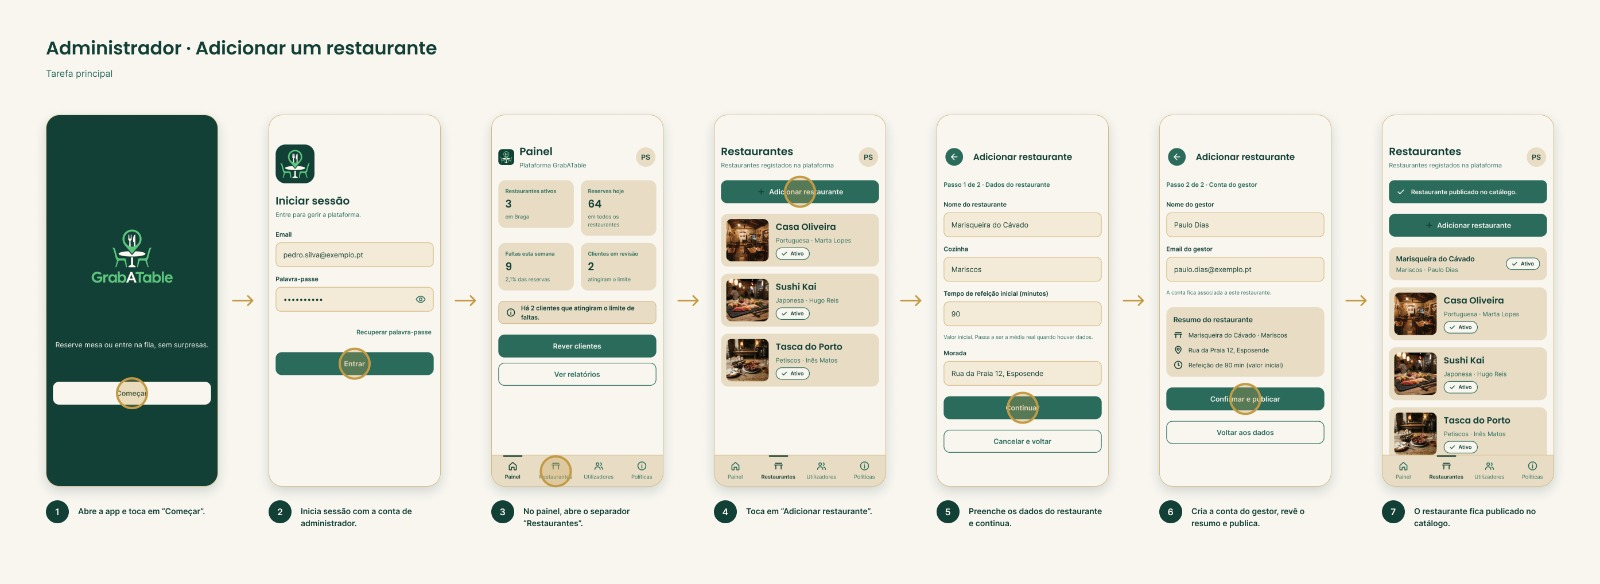
\includegraphics[width=\textwidth]{images/admin_principal.jpg}
  \caption{Administrador -- Adicionar um restaurante (tarefa principal)}
  \label{fig:proto-admin-principal}
\end{figure}

\subsubsection{Tarefa secundária -- Rever e bloquear um cliente.}
A partir do aviso no painel, o administrador abre a lista de clientes \textit{Em revisão},
consulta as faltas do cliente e confirma o bloqueio, sendo enviado um email ao cliente
(RF14). A ação é reversível através do botão \textit{Desbloquear cliente}.

\begin{figure}[H]
  \centering
  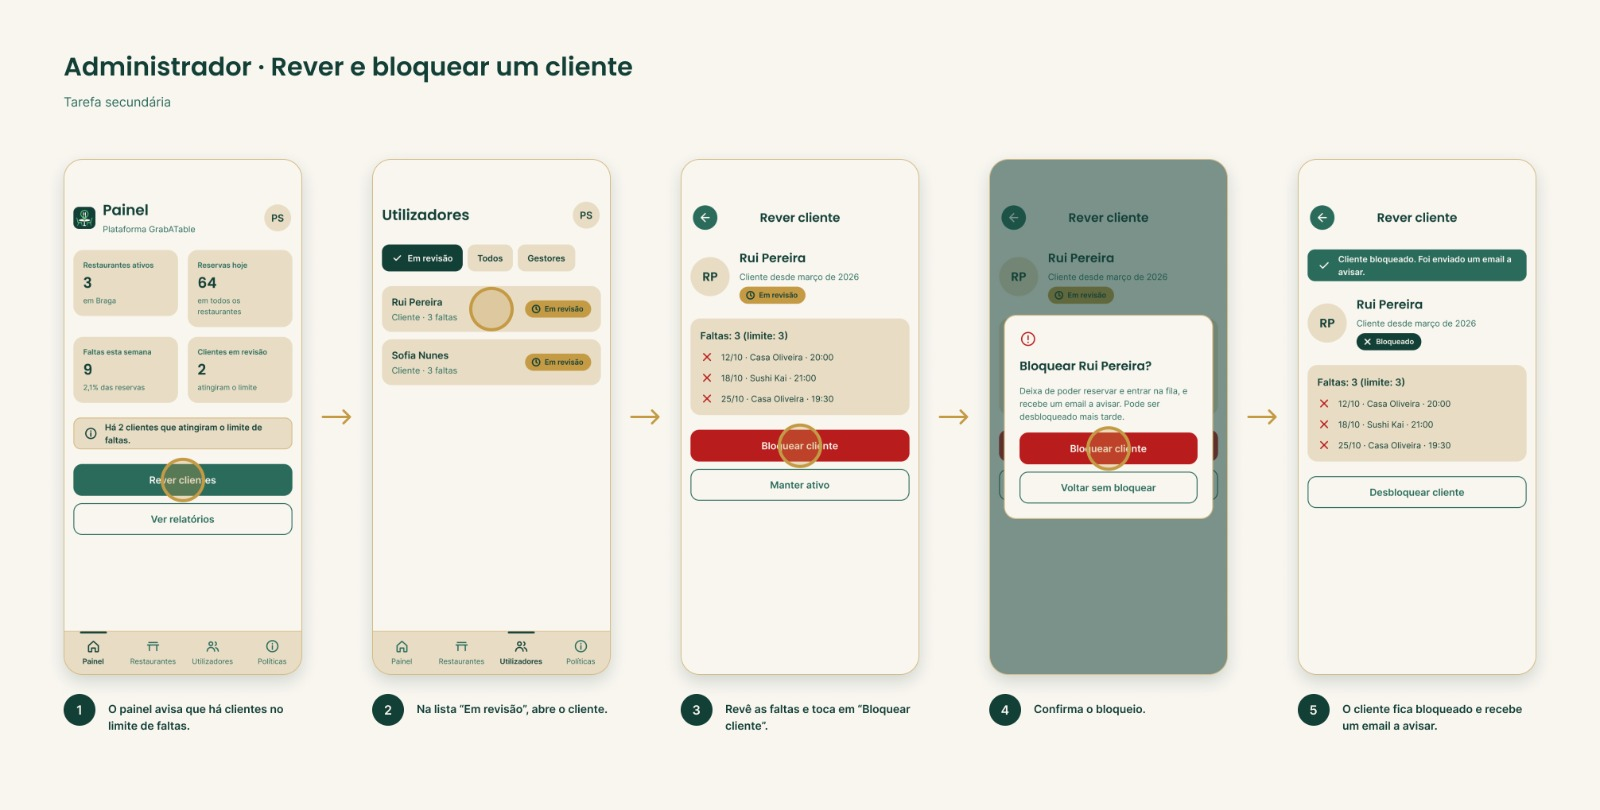
\includegraphics[width=\textwidth]{images/admin_secundario.jpg}
  \caption{Administrador -- Rever e bloquear um cliente (tarefa secundária)}
  \label{fig:proto-admin-secundario}
\end{figure}

\subsection{Gestor}

\subsubsection{Tarefa principal -- Atender um cliente com reserva.}
Corresponde ao processo de atender um cliente com reserva que foi desenhado no \textit{Task Model} principal do gestor. No painel de serviço, o gestor vê a próxima chegada, marca a chegada do cliente e confirma a mesa sugerida pelo sistema, que passa a ficar ocupada (RF09).

\begin{figure}[H]
  \centering
  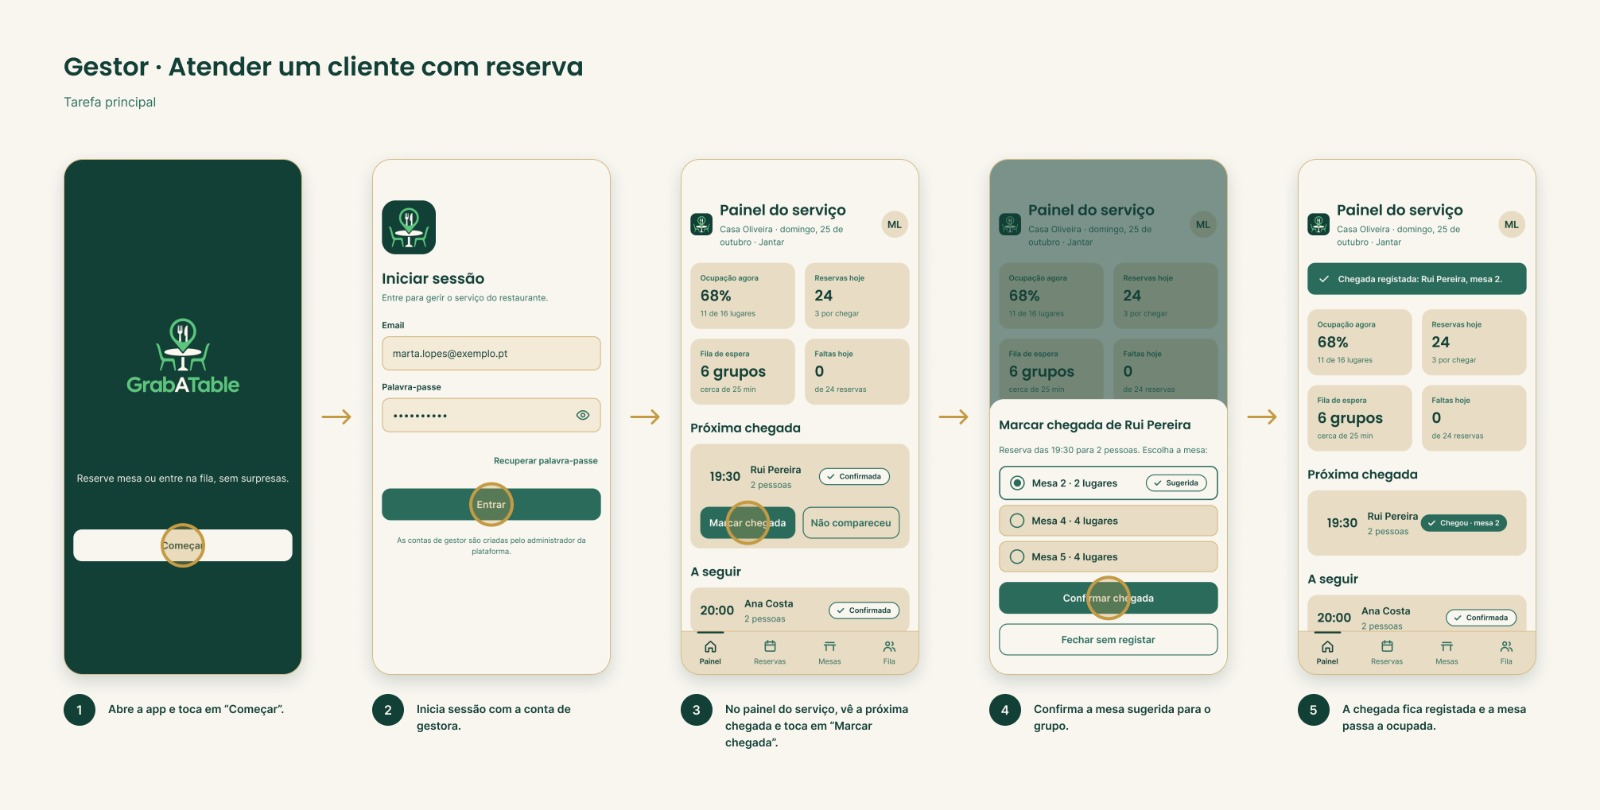
\includegraphics[width=\textwidth]{images/gestor_principal.jpg}
  \caption{Gestor -- Atender um cliente com reserva (tarefa principal)}
  \label{fig:proto-gestor-principal}
\end{figure}

\subsubsection{Tarefa secundária -- Libertar uma mesa.}
Quando o grupo sai, o gestor abre o separador \textit{Mesas} e liberta a mesa com dois
toques. O sistema avisa automaticamente o primeiro grupo da fila de espera que cabe nessa
mesa (RF10), o que mantém a estimativa de espera atualizada.

\begin{figure}[H]
  \centering
  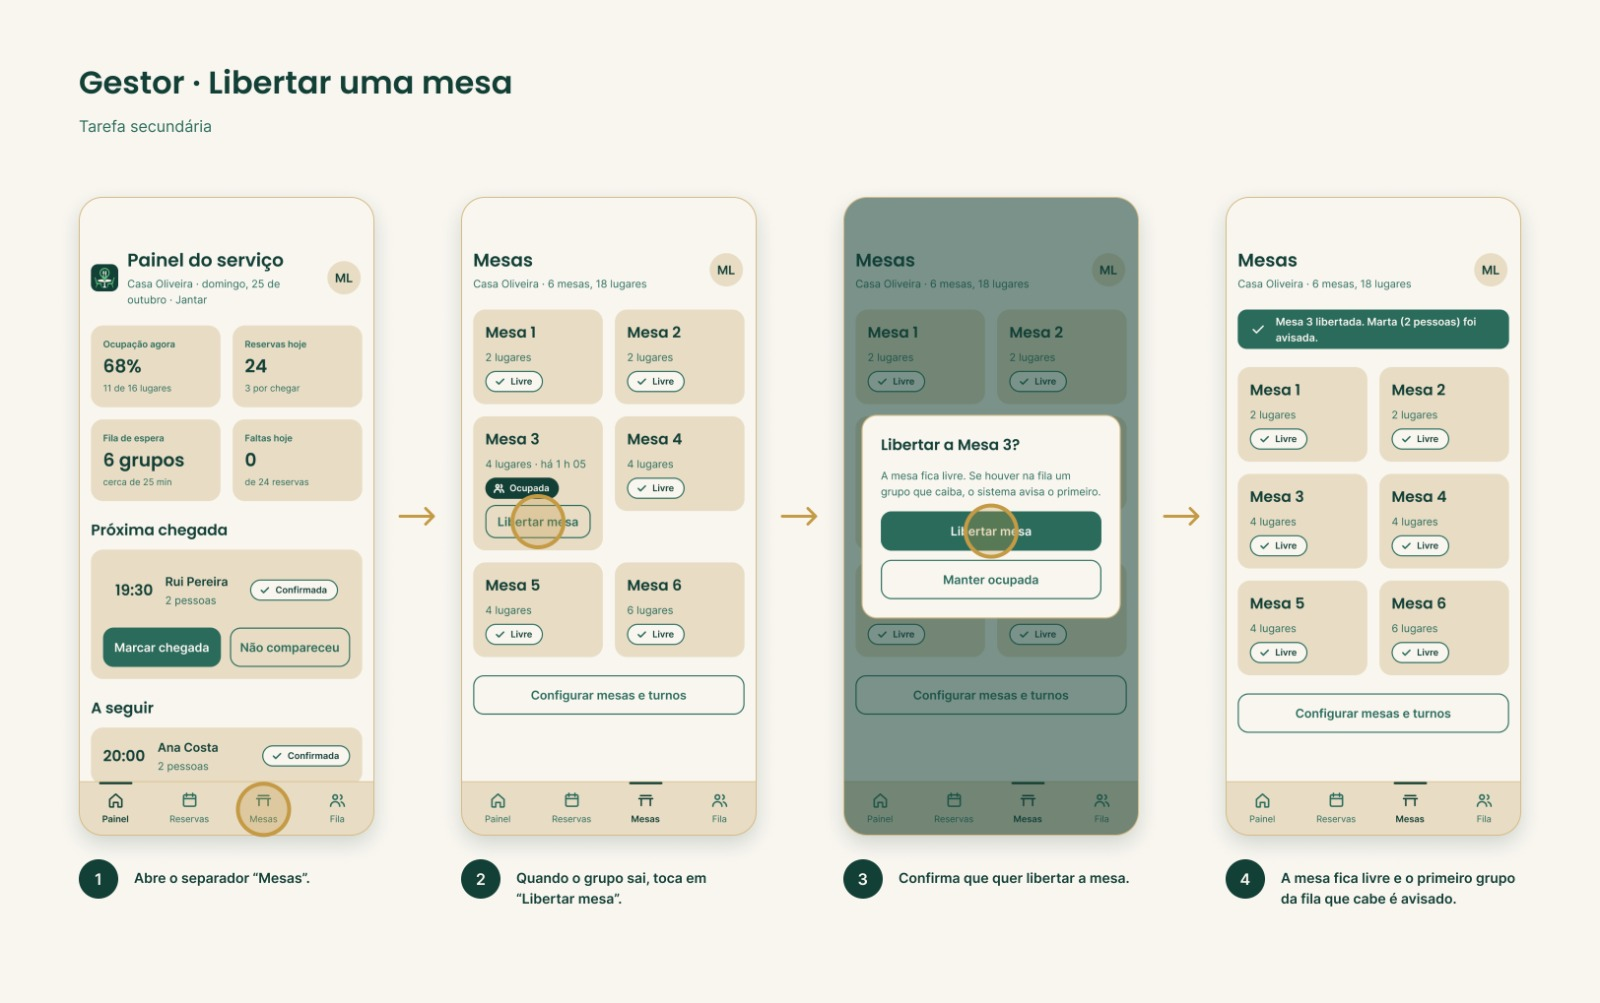
\includegraphics[width=\textwidth]{images/gestor_secundario.jpg}
  \caption{Gestor -- Libertar uma mesa (tarefa secundária)}
  \label{fig:proto-gestor-secundario}
\end{figure}

\subsection{Cliente}

\subsubsection{Tarefa principal -- Reservar mesa para refeição.}
Corresponde ao processo de reservar mesa para uma refeição que foi desenhado no \textit{Task Model} principal do cliente. O cliente inicia sessão, escolhe o restaurante, seleciona o dia, a hora e o número de pessoas e recebe a confirmação da reserva por email (RF03, RF04, RF05 e RF08).

\begin{figure}[H]
  \centering
  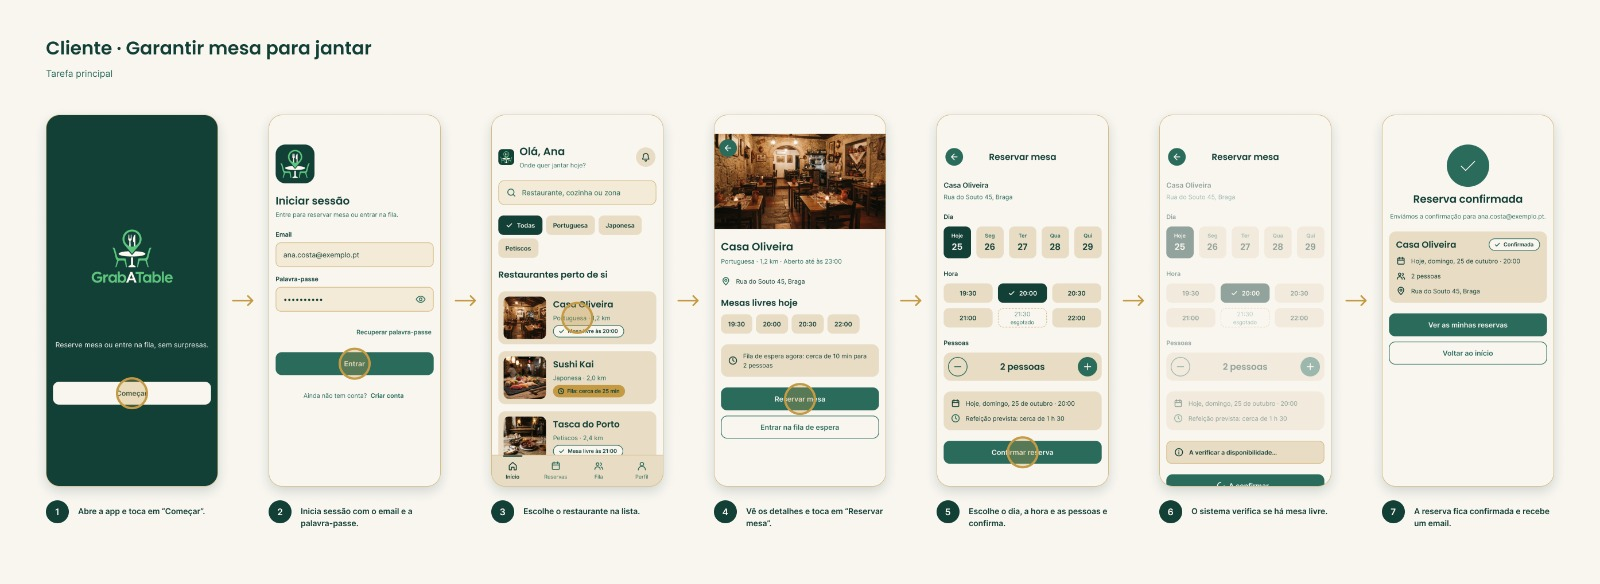
\includegraphics[width=\textwidth]{images/cliente_principal.jpg}
  \caption{Cliente -- Reservar mesa para refeição (tarefa principal)}
  \label{fig:proto-cliente-principal}
\end{figure}

\subsubsection{Tarefa secundária -- Entrar na fila de espera.}
Para o cliente sem reserva, o fluxo permite entrar na fila, ver o tempo estimado, acompanhar
a posição em tempo real e receber o aviso de que a mesa está quase pronta (RF07 e RF08).

\begin{figure}[H]
  \centering
  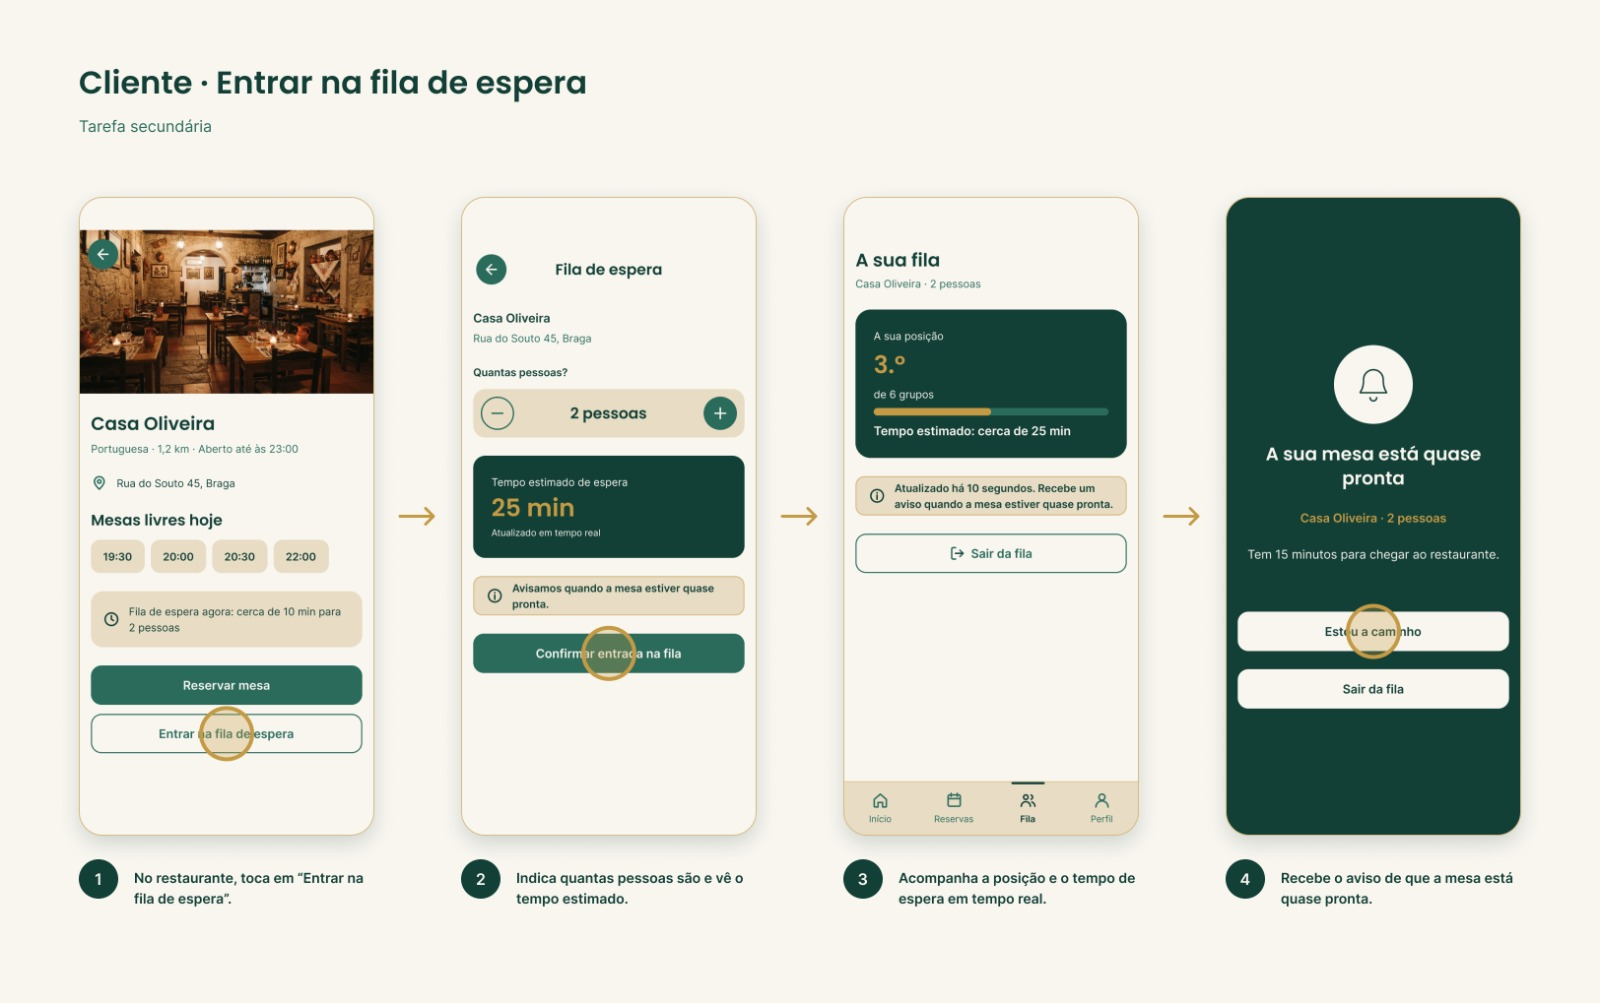
\includegraphics[width=\textwidth]{images/cliente_secundario.jpg}
  \caption{Cliente -- Entrar na fila de espera (tarefa secundária)}
  \label{fig:proto-cliente-secundario}
\end{figure}

\section{Vídeo de Demonstração}

Foi gravado um vídeo que demonstra a execução completa da tarefa principal definida para a aplicação. O vídeo está disponível em: \textit{(clicar na imagem em baixo)}

\href{https://youtube.com/shorts/b33i4PHJjyE?feature=share}{
    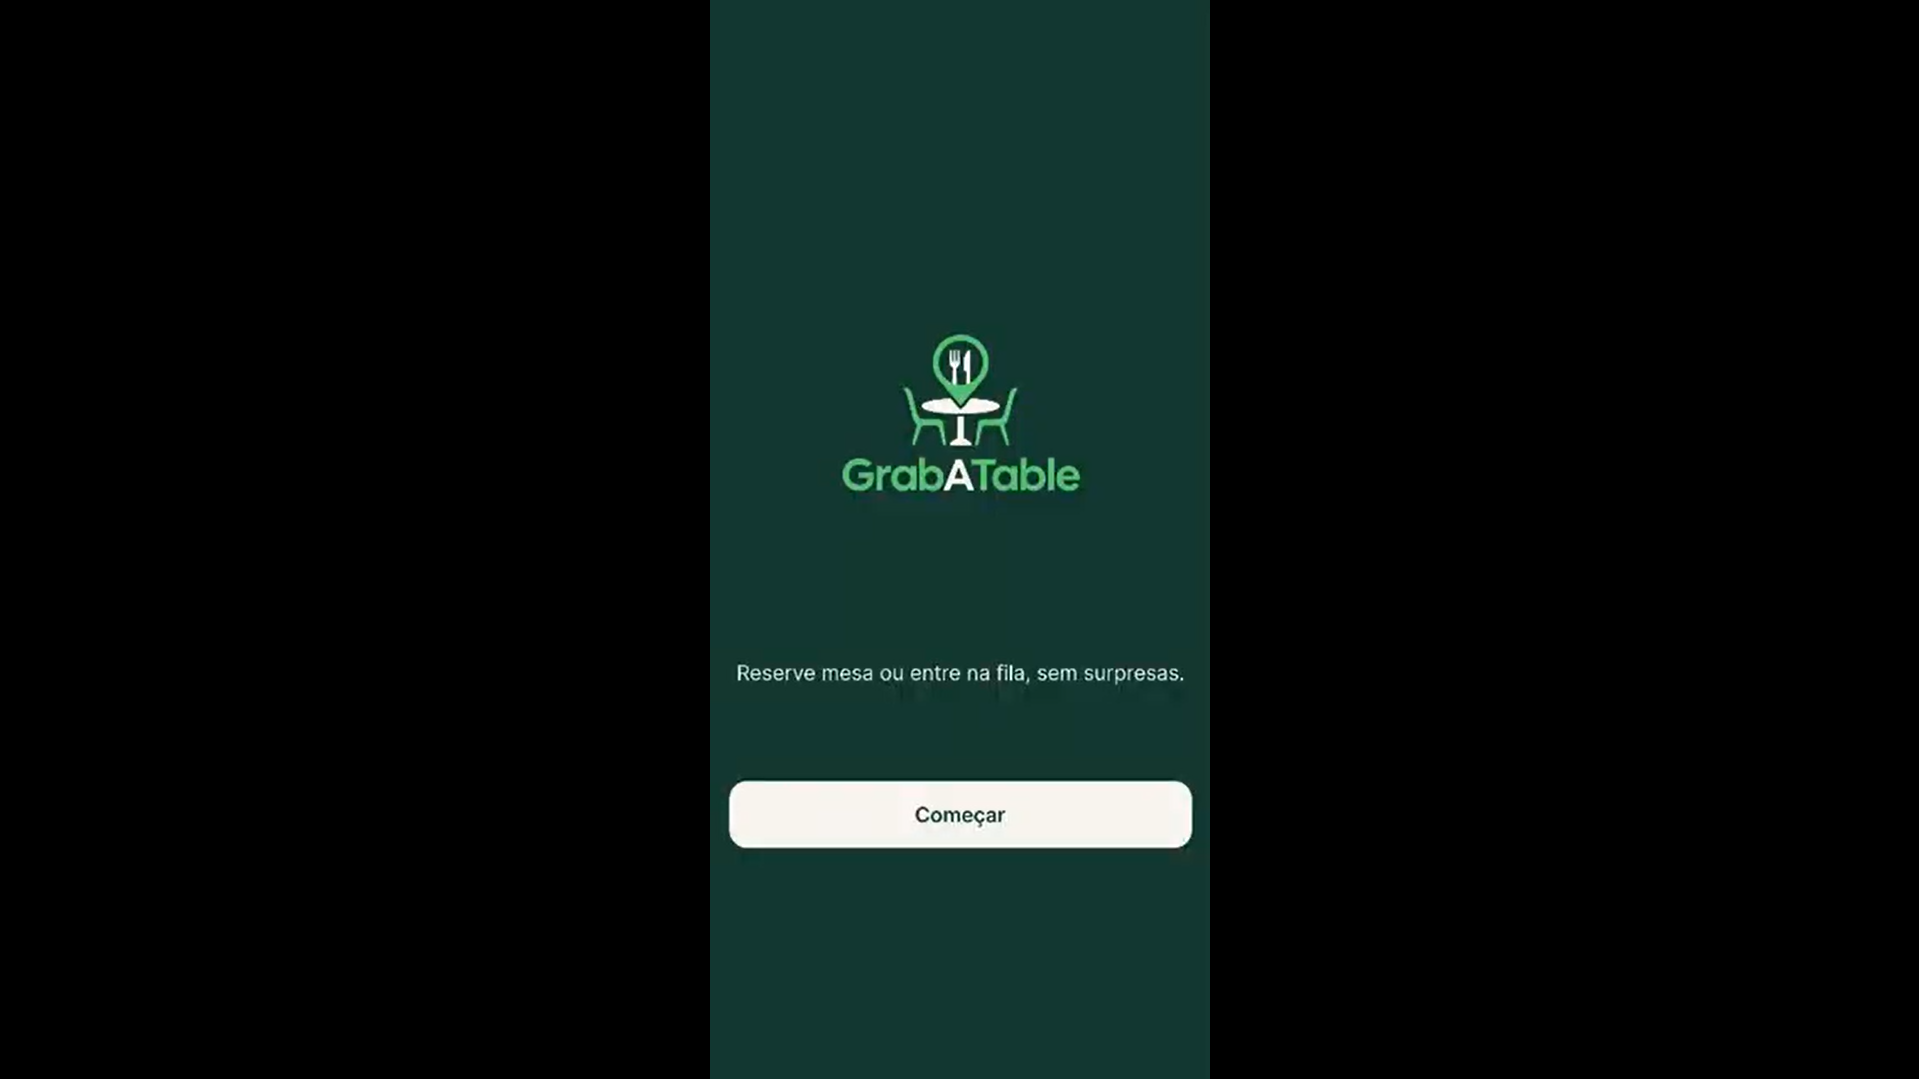
\includegraphics[width=0.9\textwidth]{images/video_foto.png}
}
% =====================================================================
% Análise heurística, problemas de usabilidade e correções
% Colocar no chap3.tex, antes de \section{Vídeo de Demonstração}:
%     \input{heuristica}
% Pacotes necessários (já tens): booktabs, longtable, array, float, graphicx
% =====================================================================
\chapter{Análise Heurística}
% --- Quadro de um problema de usabilidade (6 campos) ---
\newcommand{\problema}[6]{%
  {\small
  \begin{longtable}{>{\bfseries\raggedright\arraybackslash}p{3.3cm}
                    >{\raggedright\arraybackslash}p{\dimexpr\textwidth-3.3cm-4\tabcolsep\relax}}
    \toprule
    Ecrã ou percurso & #1 \\
    \midrule
    Descrição & #2 \\
    \midrule
    Heurística & #3 \\
    \midrule
    Consequências & #4 \\
    \midrule
    Gravidade & #5 \\
    \midrule
    Proposta de correção & #6 \\
    \bottomrule
  \end{longtable}}
}

% --- Figura de comparação (se a imagem não existir, mostra uma caixa) ---
% Uso: \figcomparacao{ficheiro.png}{legenda}{label}
\newcommand{\figcomparacao}[3]{%
  \begin{figure}[H]
    \centering
    \IfFileExists{images/#1}%
      {\includegraphics[width=\textwidth]{images/#1}}%
      {\fbox{\parbox{0.9\textwidth}{\centering\vspace{2cm}\textbf{Inserir imagem: images/#1}\vspace{2cm}}}}
    \caption{#2}
    \label{#3}
  \end{figure}
}

% =====================================================================
\section{Análise Heurística Simplificada}
\label{sec:heuristica}

A versão anterior do protótipo foi avaliada percorrendo as tarefas principais dos três perfis,
com especial atenção ao percurso do Cliente (``Garantir mesa para jantar''), e comparando cada
ecrã com as heurísticas de usabilidade abordadas nas aulas. São apresentadas apenas as heurísticas relevantes para o protótipo, com os aspetos positivos e os problemas
encontrados.

{\small
\begin{longtable}{>{\raggedright\arraybackslash}p{3cm}
                  >{\raggedright\arraybackslash}p{5.6cm}
                  >{\raggedright\arraybackslash}p{5.6cm}}
  \caption{Análise heurística da versão anterior do protótipo}\label{tab:heuristicas}\\
  \toprule
  \textbf{Heurística} & \textbf{Aspetos positivos} & \textbf{Problemas} \\
  \midrule
  \endfirsthead
  \toprule
  \textbf{Heurística} & \textbf{Aspetos positivos} & \textbf{Problemas} \\
  \midrule
  \endhead
  \bottomrule
  \endfoot

  Visibilidade do estado do sistema
  & O estado das reservas e da fila era sempre visível, através de etiquetas com texto e ícone
    (``Confirmada'', ``Cancelada'', ``Não compareceu''), e o ecrã ``A confirmar\ldots''
    informava que o pedido estava em curso.
  & Os filtros do ecrã de início e os seletores de hora e de número de pessoas não reagiam ao
    toque, pelo que o utilizador não sabia se a escolha tinha ficado registada (problema~2).
    Em vários ecrãs, o conteúdo ficava cortado no fundo, sem indicação de que havia mais
    informação (problema~1). \\
  \addlinespace

  Correspondência entre o sistema e o mundo real
  & A linguagem usa termos do dia a dia da restauração (``Reservar mesa'', ``Entrar na fila de
    espera'', ``Mesa quase pronta''). As datas, horas e números de pessoas são apresentados
    como o utilizador os diz.
  & \emph{Problema menor:} os cartões de restaurante mostravam um ícone genérico em vez de uma
    fotografia, o que dificultava reconhecer o restaurante. \\
  \addlinespace

  Controlo e liberdade do utilizador
  & As ações destrutivas (cancelar uma reserva, sair da fila) já tinham um diálogo com a opção
    de manter.
  & A barra inferior não ficava fixa e o botão voltar tinha pouco contraste (problema~3).
    Faltavam também alguns ecrãs, como a confirmação de envio da ligação de recuperação da
    palavra-passe e a eliminação da conta, o que deixava percursos sem saída. \\
  \addlinespace

  Consistência e utilização de convenções
  & A aplicação segue convenções habituais em aplicações móveis: barra de navegação inferior,
    botão voltar no canto superior esquerdo, um botão principal por ecrã.
  & Os elementos não estavam construídos como componentes reutilizáveis, o que originava
    pequenas diferenças de alinhamento e de centragem de ícones e texto entre ecrãs. \\
  \addlinespace

  Prevenção de erros
  & As horas esgotadas apareciam assinaladas antes de o utilizador as escolher.
  & Muitos elementos interativos tinham áreas de toque abaixo do mínimo recomendado, o que
    favorecia toques falhados ou no elemento errado (problema~4). \\
  \addlinespace

  Reconhecimento em vez de memorização
  & Os separadores da barra inferior combinam ícone e texto.
  & Os campos de texto tinham a mesma cor dos cartões informativos, pelo que não se
    reconheciam de imediato como zonas de escrita (problema~5). \\
  \addlinespace

  Flexibilidade e eficiência de utilização
  & O percurso principal é curto (três toques desde o ecrã de início até à reserva).
  & Os atalhos de pesquisa (filtros) não funcionavam, o que obrigava a percorrer toda a lista. \\
  \addlinespace

  Design estético e minimalista
  & Os ecrãs mostram apenas a informação necessária.
  & \emph{Problema estético:} o espaçamento vertical entre grupos de conteúdo era reduzido, o
    que tornava alguns ecrãs densos. \\
  \addlinespace

  Reconhecimento e recuperação de erros
  & Os erros de formulário (por exemplo, palavra-passe incorreta) eram apresentados junto ao
    campo, com ícone e uma mensagem que indicava como corrigir.
  & Depois de pedir a recuperação da palavra-passe, o utilizador não recebia confirmação. \\
  \addlinespace

  Ajuda e informação de apoio
  & A aplicação é simples e quase não precisa de ajuda; os campos mais exigentes têm texto de
    apoio (``Mínimo de 8 caracteres'').
  & \emph{Problema estético:} a ligação ``Política de privacidade'' no registo não levava a
    nenhum ecrã. \\
\end{longtable}}


% =====================================================================
\section{Problemas de Usabilidade}
\label{sec:problemas}

Cada problema é descrito com o ecrã ou percurso afetado, a heurística violada, as consequências
para o utilizador, a gravidade (escala de 0 a 4 de Nielsen~\cite{nielsen}) e a correção proposta.

\subsection{Problema 1: conteúdo cortado nos ecrãs longos}

\problema
  {Painel do serviço (Gestor) e, em geral, todos os ecrãs com muito conteúdo, como o Início e
   As minhas reservas.}
  {Os ecrãs não tinham \textit{scroll}, por isso todo o conteúdo tinha de caber na altura do
   telemóvel. Para isso, os elementos ficavam comprimidos: no Painel do serviço só cabiam três
   indicadores, apertados, e o texto do botão ``Não compareceu'' quase tocava na borda. As listas
   também não podiam crescer além do que cabia no ecrã.}
  {Visibilidade do estado do sistema.}
  {Informação importante ficava de fora ou difícil de ler, e as listas não podiam mostrar mais
   restaurantes ou reservas sem cortar conteúdo.}
  {3 \textperiodcentered{} Problema grave.}
  {Ativar o \textit{scroll} vertical em todos os ecrãs cujo conteúdo excede a altura do ecrã,
   mantendo fixos os elementos de navegação.}

\subsection{Problema 2: filtros e seletores sem resposta}

\problema
  {Início (filtros) e Reservar mesa (seleção de dia, hora e número de pessoas), no percurso
   principal do Cliente.}
  {Os filtros do ecrã de início (``Hoje, 20:00'', ``2 pessoas'', ``Cozinha'') e os seletores do
   ecrã de reserva não reagiam ao toque. A opção selecionada não mudava e a lista de restaurantes
   mantinha-se igual.}
  {Visibilidade do estado do sistema; Flexibilidade e eficiência de utilização.}
  {O utilizador não sabia se a escolha tinha sido registada, podia julgar que a aplicação estava
   avariada e não conseguia reduzir a lista ao tipo de cozinha pretendido.}
  {3 \textperiodcentered{} Problema grave.}
  {Tornar os seletores interativos, com estados visíveis (predefinido, selecionado, esgotado), e
   substituir os filtros por filtros de cozinha que alteram a lista apresentada.}

\subsection{Problema 3: navegação pouco persistente e botão voltar pouco visível}

\problema
  {Todos os ecrãs com barra inferior (Início, As minhas reservas, A sua fila) e todos os ecrãs
   com cabeçalho (por exemplo, Reservar mesa).}
  {A barra de navegação inferior não ficava fixa no fundo do ecrã. O botão voltar era um círculo
   bege sobre fundo creme, com pouco contraste.}
  {Controlo e liberdade do utilizador.}
  {O utilizador podia perder o acesso à navegação principal e não identificar de imediato como
   regressar ao ecrã anterior, sentindo-se ``preso''.}
  {3 \textperiodcentered{} Problema grave.}
  {Fixar a barra inferior e a barra de estado em todos os ecrãs e redesenhar o botão voltar com
   maior contraste.}

\subsection{Problema 4: áreas de toque pequenas}

\problema
  {Vários ecrãs, sobretudo Reservar mesa (opções de hora), Início (filtros) e os cabeçalhos
   (botão voltar).}
  {As ligações eram zonas desenhadas à parte, por cima de imagens importadas, e várias eram mais
   pequenas do que o botão visível, abaixo dos 44 $\times$ 44 px recomendados para ecrãs
   táteis.}
  {Prevenção de erros.}
  {Toques falhados ou no elemento ao lado, por exemplo escolher a hora errada, o que obriga o
   utilizador a repetir ações. É especialmente penalizador para quem usa o telemóvel a caminho do
   restaurante, numa só mão.}
  {3 \textperiodcentered{} Problema grave.}
  {Definir uma área de toque mínima de 44 $\times$ 44 px para todos os elementos interativos e
   aumentar o espaçamento entre eles.}

\subsection{Problema 5: campos de texto pouco reconhecíveis}

\problema
  {Iniciar sessão, Criar conta e Pesquisa, no início do percurso principal.}
  {Os campos de texto tinham a mesma cor de fundo (bege) dos cartões informativos e só se
   distinguiam deles pela borda.}
  {Reconhecimento em vez de memorização; Consistência e utilização de convenções.}
  {O utilizador demorava mais a perceber onde podia escrever, sobretudo nos formulários com
   vários campos.}
  {2 \textperiodcentered{} Problema menor.}
  {Dar aos campos de texto uma cor própria, mais clara que a dos cartões, mantendo a borda, e
   aplicá-la de forma igual em todos os campos da aplicação.}

% =====================================================================
\section{Correções e Melhorias}
\label{sec:correcoes}

Todas as correções foram feitas nos componentes do \textit{design system} do Figma. Assim, cada
alteração foi aplicada uma só vez e propagou-se automaticamente a todos os ecrãs que usam esse
componente.

\subsection{Correção 1: \textit{scroll} nos ecrãs longos}

\begin{itemize}
  \item \textbf{Problema resolvido:} problema~1.
  \item \textbf{Versão anterior:} ecrã ``Painel do serviço'' (Gestor), com três indicadores
        apertados e o botão ``Não compareceu'' no limite.
  \item \textbf{Versão corrigida:} ecrã ``31 \textperiodcentered{} Painel do serviço'', com
        quatro indicadores e \textit{scroll} vertical.
  \item \textbf{Justificação:} todos os ecrãs cujo conteúdo excede a altura do telemóvel
        passaram a ter \textit{scroll} vertical. A barra de estado e a barra inferior ficam
        fixas, para que o utilizador veja todo o conteúdo sem perder a navegação. O espaço
        inferior do conteúdo foi aumentado, para que o último elemento nunca fique escondido
        atrás da barra. Deixando de estar limitado à altura do ecrã, o painel passou a mostrar
        quatro indicadores, com espaço entre eles.
\end{itemize}

\figcomparacao{comparacao1.png}{Comparação 1: Painel do serviço antes e depois da correção}{fig:comp1}

\subsection{Correção 2: filtros e seletores interativos}

\begin{itemize}
  \item \textbf{Problema resolvido:} problema~2.
  \item \textbf{Versão anterior:} ecrãs ``Início'' e ``Reservar mesa'', com filtros e seletores
        estáticos.
  \item \textbf{Versão corrigida:} ecrãs ``06 \textperiodcentered{} Início'' e
        ``06c \textperiodcentered{} Início (Japonesa)'', com a lista filtrada, e
        ``09 \textperiodcentered{} Reservar mesa'', com os seletores interativos.
  \item \textbf{Justificação:}
    \begin{itemize}
      \item \textbf{Filtros:} passaram a ser por tipo de cozinha (Todas, Portuguesa, Japonesa,
            Petiscos); ao tocar num filtro, a lista mostra só os restaurantes dessa cozinha e o
            filtro fica assinalado;
      \item \textbf{Seletores de dia, hora e número de pessoas:} mudam de estado ao toque, com
            indicação clara da opção selecionada;
      \item \textbf{Hora esgotada:} aparece tracejada e com a palavra ``esgotado''; ao tocar
            nela, o utilizador vê uma explicação com horas alternativas.
    \end{itemize}
\end{itemize}

\figcomparacao{comparacao2.png}{Comparação 2: filtros e seletores antes e depois da correção}{fig:comp2}

\subsection{Correção 3: navegação fixa e botão voltar mais visível}

\begin{itemize}
  \item \textbf{Problema resolvido:} problema~3.
  \item \textbf{Versão anterior:} cabeçalho de ``Reservar mesa'', com o botão voltar bege, e
        ``Início'', com a barra inferior não fixa.
  \item \textbf{Versão corrigida:} os mesmos ecrãs, com o botão voltar verde e a barra inferior
        fixa.
  \item \textbf{Justificação:}
    \begin{itemize}
      \item \textbf{Barra inferior:} fica sempre visível, com o separador ativo assinalado por um
            indicador e texto em negrito;
      \item \textbf{Botão voltar:} passou a ser um círculo verde com seta creme, com um contraste
            de 5,8:1, no mesmo sítio em todos os ecrãs;
      \item \textbf{Ecrãs em falta:} acrescentaram-se os ecrãs que faltavam (confirmação do envio
            da ligação de recuperação, política de privacidade, alteração da fotografia e
            eliminação da conta), para que nenhum percurso fique sem saída.
    \end{itemize}
\end{itemize}

\figcomparacao{comparacao3.png}{Comparação 3: navegação e botão voltar antes e depois da correção}{fig:comp3}

\subsection{Correção 4: áreas de toque com o mínimo recomendado}

\begin{itemize}
  \item \textbf{Problema resolvido:} problema~4.
  \item \textbf{Versão anterior:} ecrã ``Reservar mesa'', com as ligações em zonas desenhadas à
        parte, mais pequenas do que os botões.
  \item \textbf{Versão corrigida:} componentes com as novas dimensões, por exemplo no ecrã
        ``09 \textperiodcentered{} Reservar mesa''.
  \item \textbf{Justificação:} todos os elementos interativos passaram a ter pelo menos
        44 $\times$ 44 px:
    \begin{itemize}
      \item botões: 52 px de altura;
      \item opções de hora e filtros: 44 px;
      \item botão voltar, avatar e sino: 48 $\times$ 48 px;
      \item itens da barra inferior: 97,5 $\times$ 72 px.
    \end{itemize}
    O espaço entre grupos de conteúdo passou para 24 px, o que também reduz toques no elemento
    errado. As dimensões foram verificadas em todos os elementos com ligação no protótipo.
\end{itemize}

\figcomparacao{comparacao4.png}{Comparação 4: áreas de toque antes e depois da correção}{fig:comp4}

\subsection{Correção 5: campos de texto com cor própria}

\begin{itemize}
  \item \textbf{Problema resolvido:} problema~5.
  \item \textbf{Versão anterior:} ecrã ``Iniciar sessão'', com os campos em bege, iguais aos
        cartões.
  \item \textbf{Versão corrigida:} ecrã ``02 \textperiodcentered{} Iniciar sessão'', com os
        campos em bege claro (\autoref{fig:comp5}).
  \item \textbf{Justificação:} acrescentou-se à paleta uma nova cor, o bege claro
        (\texttt{\#F3EAD7}), usada em todos os campos de texto e na pesquisa, mantendo a borda
        em areia. Os campos distinguem-se assim dos cartões informativos. O texto escrito mantém
        um contraste de 9,8:1, acima do nível AA da WCAG~\cite{wcag}.
\end{itemize}

\figcomparacao{comparacao5.png}{Comparação 5: campos de texto antes e depois da correção}{fig:comp5}

\subsection{Outras melhorias}

Além dos cinco problemas descritos, a análise motivou outras alterações:

\begin{itemize}
  \item \textbf{Fotografias:} os cartões e os detalhes de restaurante passaram a mostrar
        fotografias;
  \item \textbf{Ecrã de abertura:} passou a existir em todos os percursos, incluindo os do Gestor
        e do Administrador;
  \item \textbf{Organização no Figma:} os componentes ficaram agrupados num \textit{design
        system}, com nomes claros e variantes de estado, e os ecrãs em secções por percurso;
  \item \textbf{Fidelidade ao sistema visual:} confirmou-se que as cores, a tipografia, a grelha
        e as margens do protótipo correspondem ao definido na \autoref{sec:sistema-visual}.
\end{itemize}
\chapter{Resiliência e Observabilidade}
\label{cap:resiliencia}

Numa arquitetura de microsserviços, a falha de uma peça é uma situação normal e não uma
exceção. Este capítulo descreve como a plataforma se comporta quando um serviço, uma
dependência, a base de dados ou o \textit{broker} de mensagens falham, que respostas recebe a
aplicação, e como se acompanha cada pedido de ponta a ponta.

\section{Princípios}

\begin{itemize}
  \item \textbf{Isolamento:} cada serviço tem a sua base de dados e o seu processo; a falha de um
        serviço não impede os outros de responder;
  \item \textbf{Comunicação assíncrona:} os serviços avisam-se por eventos no RabbitMQ~\cite{rabbitmq}. Se o
        consumidor estiver em baixo, o evento fica na fila e é processado quando o serviço
        volta. É o que garante o RNF04: uma falha no serviço de notificações não impede a criação de reservas;
  \item \textbf{Autenticação sem dependências:} o JWT é validado localmente no gateway e em cada
        serviço; sem o serviço de autenticação deixa de ser possível iniciar sessão, mas os
        tokens já emitidos continuam válidos;
  \item \textbf{Falhar depressa e com clareza:} uma dependência em baixo dá uma resposta 503 com uma
        mensagem que explica o que falhou, em vez de um erro genérico ou de um pedido pendurado.
\end{itemize}

\section{Respostas de Erro}

Todas as respostas de erro seguem o formato \textit{Problem Details} (RFC 9457) e estão em
português, incluindo as que o ASP.NET Core gera automaticamente (falta de token, validação dos
campos, JSON mal formado). Cada resposta indica o serviço que produziu o erro (\texttt{service})
e o identificador do pedido (\texttt{traceId}), que permite encontrá-lo nos registos e no
Jaeger. Por exemplo, com o serviço de reservas parado:

\begin{verbatim}
HTTP/1.1 503 Service Unavailable
X-Trace-Id: b289140cbcf9c7ea82409207641383cd
{
  "title": "Serviço indisponível",
  "status": 503,
  "detail": "O serviço de reservas está indisponível.",
  "service": "reservations",
  "traceId": "00-b289140cbcf9c7ea82409207641383cd-ed21d1c051186c8d-01"
}
\end{verbatim}

\begin{table}[H]
\centering
\begin{tabularx}{\textwidth}{lX}
\toprule
\textbf{Código} & \textbf{Quando} \\
\midrule
400 & Dados inválidos, com a lista de erros por campo \\
401 & Sem sessão iniciada: token em falta, inválido ou expirado \\
403 & Perfil sem permissão, ou gestor a atuar noutro restaurante \\
404 & Recurso inexistente (ou de outro cliente) \\
409 & Conflito: reserva repetida, mesa já livre, sem mesas para a hora pedida \\
422 & Pedido impossível: nenhuma mesa serve o grupo \\
429 & Demasiados pedidos nas rotas públicas do Auth \\
503 & Serviço, base de dados ou RabbitMQ indisponíveis \\
504 & Um serviço não respondeu a tempo ao gateway \\
\bottomrule
\end{tabularx}
\caption{Códigos de erro devolvidos à aplicação}
\label{tab:codigos}
\end{table}

\section{Resiliência na Comunicação Síncrona}
\label{sec:resiliencia-http}

A chamada do serviço de reservas ao serviço de restaurantes é a única dependência síncrona entre
serviços, e por isso é protegida com três mecanismos:

\begin{itemize}
  \item \textbf{Tempo limite:} cada tentativa tem no máximo 2 segundos (8 segundos no total);
  \item \textbf{Novas tentativas:} até duas, para falhas transitórias;
  \item Se pelo menos metade de quatro ou mais chamadas falhar num intervalo de 10 segundos, o circuito abre durante 15 segundos. Enquanto está aberto, os pedidos falham imediatamente, sem esperar por um serviço que se sabe estar em baixo, o que evita acumular pedidos pendurados e consumir recursos.
\end{itemize}

\section{Comportamento em Caso de Falhas}

Os cenários seguintes foram executados no ambiente completo (Docker Compose), parando um
container de cada vez. Estão automatizados numa \textit{collection} do Postman própria. Os tempos indicados foram medidos.

\begin{table}[H]
\centering
\small
\begin{tabularx}{\textwidth}{lXX}
\toprule
\textbf{Peça parada} & \textbf{Resposta à aplicação} & \textbf{O que demonstra} \\
\midrule
Serviço de reservas &
503 do gateway: ``O serviço de reservas está indisponível.'' Os restantes serviços continuam
a responder normalmente. &
Isolamento entre serviços; o gateway responde com clareza em vez de um 502 sem corpo. \\
\midrule
Serviço de autenticação &
Login: 503. Pedidos com um token já emitido: 200. &
O JWT é validado localmente: o sistema continua a funcionar para quem já tem sessão. \\
\midrule
Serviço de restaurantes &
Reservar: 503 do serviço de reservas. 1.\textsuperscript{a} tentativa em cerca de 6,7~s
(tentativas com tempo limite), 2.\textsuperscript{a} em cerca de 2~s, a partir da
3.\textsuperscript{a} em menos de 20~ms. ``As minhas reservas'' continua a
funcionar. &
Tempo limite e novas tentativas; só falham as operações que dependem do serviço em
baixo. \\
\midrule
Serviço de notificações &
A reserva é criada (201). Ao voltar, o serviço processa o evento que ficou na fila e a
notificação aparece. &
Comunicação assíncrona e consistência eventual (RNF04). \\
\midrule
PostgreSQL &
503: ``A base de dados do serviço de restaurantes está indisponível.'' &
Falhas de infraestrutura distinguem-se de erros do pedido. \\
\midrule
RabbitMQ &
Reservar: 503 ao fim de 5~s: ``a alteração foi gravada, mas os outros serviços não foram
avisados''. Ao voltar, os serviços religam-se sozinhos em 20 a 40~s. &
Limitação conhecida (Secção~\ref{sec:limitacoes}). \\
\bottomrule
\end{tabularx}
\caption{Comportamento do sistema com cada peça parada}
\label{tab:falhas}
\end{table}

\section{Limitações Conhecidas}
\label{sec:limitacoes}

Cada serviço grava a alteração na sua base de dados e só depois publica o evento. Se o RabbitMQ
estiver em baixo nesse momento, a alteração fica gravada mas os outros serviços não são avisados:
por exemplo, a reserva existe, mas a fila de espera e as notificações nunca recebem o evento de
confirmação. O sistema deteta a situação e responde 503 ao fim de 5 segundos, em vez de deixar
o pedido pendurado, mas a inconsistência mantém-se.

A solução é o padrão \textit{transactional outbox}: o evento é gravado numa tabela da mesma base de
dados, na mesma transação da alteração, e um processo em segundo plano publica-o quando o
RabbitMQ estiver disponível. O MassTransit oferece esta funcionalidade para o Entity Framework
Core; fica como trabalho futuro, porque exige tabelas novas nos cinco serviços.

\chapter{Resiliência e Observabilidade}
\label{cap:resiliencia}

Numa arquitetura de microsserviços, a falha de uma peça é uma situação normal e não uma
exceção. Este capítulo descreve como a plataforma se comporta quando um serviço, uma
dependência, a base de dados ou o \textit{broker} de mensagens falham, que respostas recebe a
aplicação, e como se acompanha cada pedido de ponta a ponta.

\section{Princípios}

\begin{itemize}
  \item \textbf{Isolamento:} cada serviço tem a sua base de dados e o seu processo; a falha de um
        serviço não impede os outros de responder;
  \item \textbf{Comunicação assíncrona:} os serviços avisam-se por eventos no RabbitMQ~\cite{rabbitmq}. Se o
        consumidor estiver em baixo, o evento fica na fila e é processado quando o serviço
        volta. É o que garante o RNF04: uma falha no serviço de notificações não impede a criação de reservas;
  \item \textbf{Autenticação sem dependências:} o JWT~\cite{rfc7519} é validado localmente no gateway e em cada
        serviço; sem o serviço de autenticação deixa de ser possível iniciar sessão, mas os
        tokens já emitidos continuam válidos;
  \item \textbf{Falhar depressa e com clareza:} uma dependência em baixo dá uma resposta 503 com uma
        mensagem que explica o que falhou, em vez de um erro genérico ou de um pedido pendurado.
\end{itemize}

\section{Respostas de Erro}

Todas as respostas de erro seguem o formato \textit{Problem Details} (RFC 9457) e estão em
português, incluindo as que o ASP.NET Core~\cite{dotnet,aspnetcore} gera automaticamente (falta de token, validação dos
campos, JSON mal formado). Cada resposta indica o serviço que produziu o erro (\texttt{service})
e o identificador do pedido (\texttt{traceId}), que permite encontrá-lo nos registos e no
Jaeger~\cite{jaeger}. Por exemplo, com o serviço de reservas parado:

\begin{verbatim}
HTTP/1.1 503 Service Unavailable
X-Trace-Id: b289140cbcf9c7ea82409207641383cd
{
  "title": "Serviço indisponível",
  "status": 503,
  "detail": "O serviço de reservas está indisponível.",
  "service": "reservations",
  "traceId": "00-b289140cbcf9c7ea82409207641383cd-ed21d1c051186c8d-01"
}
\end{verbatim}

\begin{table}[H]
\centering
\begin{tabularx}{\textwidth}{lX}
\toprule
\textbf{Código} & \textbf{Quando} \\
\midrule
400 & Dados inválidos, com a lista de erros por campo \\
401 & Sem sessão iniciada: token em falta, inválido ou expirado \\
403 & Perfil sem permissão, ou gestor a atuar noutro restaurante \\
404 & Recurso inexistente (ou de outro cliente) \\
409 & Conflito: reserva repetida, mesa já livre, sem mesas para a hora pedida \\
422 & Pedido impossível: nenhuma mesa serve o grupo \\
429 & Demasiados pedidos nas rotas públicas do Auth \\
503 & Serviço, base de dados ou RabbitMQ~\cite{rabbitmq} indisponíveis \\
504 & Um serviço não respondeu a tempo ao gateway \\
\bottomrule
\end{tabularx}
\caption{Códigos de erro devolvidos à aplicação}
\label{tab:codigos}
\end{table}

\section{Resiliência na Comunicação Síncrona}
\label{sec:resiliencia-http}

A chamada do serviço de reservas ao serviço de restaurantes é a única dependência síncrona entre
serviços, e por isso é protegida com três mecanismos:

\begin{itemize}
  \item \textbf{Tempo limite:} cada tentativa tem no máximo 2 segundos (8 segundos no total);
  \item \textbf{Novas tentativas:} até duas, para falhas transitórias;
  \item Se pelo menos metade de quatro ou mais chamadas falhar num intervalo de 10 segundos, o circuito abre durante 15 segundos. Enquanto está aberto, os pedidos falham imediatamente, sem esperar por um serviço que se sabe estar em baixo, o que evita acumular pedidos pendurados e consumir recursos.
\end{itemize}

\section{Comportamento em Caso de Falhas}

Os cenários seguintes foram executados no ambiente completo (Docker Compose)~\cite{compose}, parando um
container de cada vez. Estão automatizados numa \textit{collection} do Postman~\cite{postman} própria. Os tempos indicados foram medidos.

\begin{table}[H]
\centering
\small
\begin{tabularx}{\textwidth}{lXX}
\toprule
\textbf{Serviço parado} & \textbf{Resposta à aplicação} & \textbf{O que demonstra} \\
\midrule
Serviço de reservas &
503 do gateway: ``O serviço de reservas está indisponível.'' Os restantes serviços continuam
a responder normalmente. &
Isolamento entre serviços; o gateway responde com clareza em vez de um 502 sem corpo. \\
\midrule
Serviço de autenticação &
Login: 503. Pedidos com um token já emitido: 200. &
O JWT~\cite{rfc7519} é validado localmente: o sistema continua a funcionar para quem já tem sessão. \\
\midrule
Serviço de restaurantes &
Reservar: 503 do serviço de reservas. 1.\textsuperscript{a} tentativa em cerca de 6,7~s
(tentativas com tempo limite), 2.\textsuperscript{a} em cerca de 2~s, a partir da
3.\textsuperscript{a} em menos de 20~ms. ``As minhas reservas'' continua a
funcionar. &
Tempo limite e novas tentativas; só falham as operações que dependem do serviço em
baixo. \\
\midrule
Serviço de notificações &
A reserva é criada (201). Ao voltar, o serviço processa o evento que ficou na fila e a
notificação aparece. &
Comunicação assíncrona e consistência eventual (RNF04). \\
\midrule
PostgreSQL &
503: ``A base de dados do serviço de restaurantes está indisponível.'' &
Falhas de infraestrutura distinguem-se de erros do pedido. \\
\midrule
RabbitMQ &
Reservar: 503 ao fim de 5~s: ``a alteração foi gravada, mas os outros serviços não foram
avisados''. Ao voltar, os serviços religam-se sozinhos em 20 a 40~s. &
Limitação conhecida (Secção~\ref{sec:limitacoes}). \\
\bottomrule
\end{tabularx}
\caption{Comportamento do sistema com cada peça parada}
\label{tab:falhas}
\end{table}

\section{Limitações Conhecidas}
\label{sec:limitacoes}

Cada serviço grava a alteração na sua base de dados e só depois publica o evento. Se o RabbitMQ~\cite{rabbitmq}
estiver em baixo nesse momento, a alteração fica gravada mas os outros serviços não são avisados:
por exemplo, a reserva existe, mas a fila de espera e as notificações nunca recebem o evento de
confirmação. O sistema deteta a situação e responde 503 ao fim de 5 segundos, em vez de deixar
o pedido pendurado, mas a inconsistência mantém-se.

A solução é o padrão \textit{transactional outbox}: o evento é gravado numa tabela da mesma base de
dados, na mesma transação da alteração, e um processo em segundo plano publica-o quando o
RabbitMQ~\cite{rabbitmq} estiver disponível. O MassTransit oferece esta funcionalidade para o Entity Framework
Core; fica como trabalho futuro, porque exige tabelas novas nos cinco serviços.

\section{Requisitos Cumpridos}

A Tabela~\ref{tab:rastreabilidade} relaciona cada requisito definido na Secção~2.3 com a sua
implementação.

\begin{longtable}{p{0.09\textwidth}p{0.13\textwidth}p{0.66\textwidth}}
\label{tab:rastreabilidade} \\
\toprule
\textbf{Req.} & \textbf{Estado} & \textbf{Implementação} \\
\midrule
\endfirsthead
\toprule
\textbf{Req.} & \textbf{Estado} & \textbf{Implementação} \\
\midrule
\endhead
\bottomrule
\endfoot
RF01 & Cumprido & Registo de clientes e login (Auth); gestores criados pelo administrador \\
RF02 & Cumprido & Recuperação de palavra-passe com ligação por email (Auth e Notifications) \\
RF03 & Cumprido & Pesquisa por texto (nome, cozinha, cidade), cozinha, data e número de pessoas;
a hora escolhe-se na disponibilidade (Restaurants) \\
RF04 & Cumprido & Detalhes do restaurante e horas disponíveis, incluindo as esgotadas
(Restaurants e Reservations) \\
RF05 & Cumprido & Reserva com data, hora e número de pessoas, sem exceder as mesas \\
RF06 & Cumprido & Consultar (próximas e histórico), alterar e cancelar reservas \\
RF07 & Cumprido & Entrar e sair da fila, posição, total de grupos e tempo estimado \\
RF08 & Cumprido & Emails de reserva confirmada, alterada e cancelada e de mesa disponível para o
grupo da fila (Notifications) \\
RF09 & Cumprido & Reservas do restaurante, reservas manuais, chegada com sugestão de mesa e não
comparência \\
RF10 & Cumprido & Fila do restaurante, chamar o próximo grupo que cabe e atribuição automática de
mesas livres \\
RF11 & Cumprido & Mesas, capacidades, turnos, horários e tempo médio de refeição \\
RF12 & Parcial & Ocupação por dia e tempo médio de refeição real (Restaurants); taxa de faltas
nos relatórios do administrador. Faltam estatísticas dos tempos de espera da fila \\
RF13 & Cumprido & Criar e editar restaurantes; remover é feito por desativação, para manter o
histórico \\
RF14 & Cumprido & Lista de utilizadores com filtros, bloqueio e desbloqueio; os clientes que
atingem o limite de faltas ficam marcados para revisão \\
RF15 & Cumprido & Limite de faltas (Auth) e tempo de refeição, margem e tolerância por defeito
(Restaurants) \\
RF16 & Cumprido & Reservas e taxa de faltas por restaurante ou por região \\
RF17 & Cumprido & Alterar palavra-passe e fotografia de perfil \\
\midrule
RNF01 & Por medir & Estimativa atualizada por eventos, em menos de um segundo após cada alteração;
não foram feitos testes de carga para medir o percentil 95 \\
RNF02 & Parcial & JWT~\cite{rfc7519} validado no gateway e em cada serviço, BCrypt~\cite{bcrypt}, controlo de acesso por perfil.
O ambiente local usa HTTP; o HTTPS fica a cargo do ponto de entrada em produção \\
RNF03 & Cumprido & Só o gateway publica uma porta; serviços, base de dados e RabbitMQ~\cite{rabbitmq} na rede
interna \\
RNF04 & Cumprido & Comunicação assíncrona; demonstrado com o serviço de notificações parado
(Tabela~\ref{tab:falhas}) \\
RNF05 & Cumprido & Os microsserviços devem ser executados em containers Docker~\cite{docker} e não guardar estado em memória: os dados ficam na respetiva base de dados PostgreSQL~\cite{postgresql} e as mensagens no RabbitMQ~\cite{rabbitmq}.\\
RNF06 & Cumprido & Um serviço e uma base de dados por área de negócio, \textit{migrations}
versionadas e OpenAPI~\cite{openapi} de cada serviço \\
RNF07 & Protótipo & Abordagem \textit{mobile first} definida no protótipo de alta fidelidade; a
aplicação cliente não fez parte da implementação \\
RNF08 & Cumprido & 114 testes unitários e de integração e duas \textit{collections} do Postman~\cite{postman}
(Capítulo~\ref{cap:testes}) \\
RNF09 & Cumprido & Consentimento no registo e eliminação de conta com anonimização em todos os
serviços \\
\caption{Rastreabilidade dos requisitos}
\end{longtable}
\chapter{Containers -- Docker}
\label{cap:implantacao}

\section{Imagens}

Todos os serviços usam o mesmo \textit{Dockerfile}, em duas fases e com imagens oficiais da
Microsoft: a compilação é feita na imagem do SDK do .NET 10 e o resultado é copiado para a imagem
\texttt{aspnet:10.0}, mais pequena e sem ferramentas de compilação. O processo corre com um
utilizador sem privilégios de administrador. O PostgreSQL, o RabbitMQ e o Jaeger usam também as
imagens oficiais.

\section{Ambiente com Docker Compose}

O ficheiro \texttt{deploy/docker-compose.yml} arranca o ambiente completo com um só comando:

\begin{verbatim}
docker compose --env-file .env -f deploy/docker-compose.yml up -d --build
\end{verbatim}

\begin{table}[H]
\centering
\small
\renewcommand{\arraystretch}{1.2}
\begin{tabularx}{\textwidth}{>{\raggedright\arraybackslash}p{0.28\textwidth} X}
\toprule
\textbf{Container} & \textbf{Função} \\
\midrule
\texttt{gateway} & API Gateway; único com porta publicada (8080) \\
\texttt{auth-api}, \texttt{restaurants-api}, \texttt{reservations-api}, \texttt{waitlist-api}, \texttt{notifications-api}
& Microsserviços, apenas na rede interna \\
\texttt{postgres}
& PostgreSQL 17; um \textit{script} de arranque cria as cinco bases de dados e um utilizador só de leitura para exportação de dados \\
\texttt{rabbitmq}
& \textit{Broker} de mensagens \\
\texttt{jaeger}
& Rastreio distribuído; interface apenas acessível na própria máquina \\
\bottomrule
\end{tabularx}
\caption{Containers do ambiente}
\label{tab:containeres}
\end{table}

Os serviços só arrancam depois de o PostgreSQL e o RabbitMQ estarem prontos, e cada serviço aplica as suas \textit{migrations} ao arrancar. As credenciais e a
chave do JWT vêm de um ficheiro \texttt{.env} que nunca é guardado no repositório; o repositório
inclui apenas um \texttt{.env.example}. Em ambiente de desenvolvimento, os serviços criam os dados de
exemplo do protótipo (três restaurantes em Braga e as contas de cliente, gestora e administrador).

\chapter{Conclusão e Trabalho Futuro}
\label{cap:conclusao}

\section{Requisitos Cumpridos}

A Tabela~\ref{tab:rastreabilidade} relaciona cada requisito definido na Secção~2.3 com a sua
implementação.

\begin{longtable}{p{0.09\textwidth}p{0.13\textwidth}p{0.66\textwidth}}
\label{tab:rastreabilidade} \\
\toprule
\textbf{Req.} & \textbf{Estado} & \textbf{Implementação} \\
\midrule
\endfirsthead
\toprule
\textbf{Req.} & \textbf{Estado} & \textbf{Implementação} \\
\midrule
\endhead
\bottomrule
\endfoot
RF01 & Cumprido & Registo de clientes e login (Auth); gestores criados pelo administrador \\
RF02 & Cumprido & Recuperação de palavra-passe com ligação por email (Auth e Notifications) \\
RF03 & Cumprido & Pesquisa por texto (nome, cozinha, cidade), cozinha, data e número de pessoas;
a hora escolhe-se na disponibilidade (Restaurants) \\
RF04 & Cumprido & Detalhes do restaurante e horas disponíveis, incluindo as esgotadas
(Restaurants e Reservations) \\
RF05 & Cumprido & Reserva com data, hora e número de pessoas, sem exceder as mesas \\
RF06 & Cumprido & Consultar (próximas e histórico), alterar e cancelar reservas \\
RF07 & Cumprido & Entrar e sair da fila, posição, total de grupos e tempo estimado \\
RF08 & Cumprido & Emails de reserva confirmada, alterada e cancelada e de mesa disponível para o
grupo da fila (Notifications) \\
RF09 & Cumprido & Reservas do restaurante, reservas manuais, chegada com sugestão de mesa e não
comparência \\
RF10 & Cumprido & Fila do restaurante, chamar o próximo grupo que cabe e atribuição automática de
mesas livres \\
RF11 & Cumprido & Mesas, capacidades, turnos, horários e tempo médio de refeição \\
RF12 & Parcial & Ocupação por dia e tempo médio de refeição real (Restaurants); taxa de faltas
nos relatórios do administrador. Faltam estatísticas dos tempos de espera da fila \\
RF13 & Cumprido & Criar e editar restaurantes; remover é feito por desativação, para manter o
histórico \\
RF14 & Cumprido & Lista de utilizadores com filtros, bloqueio e desbloqueio; os clientes que
atingem o limite de faltas ficam marcados para revisão \\
RF15 & Cumprido & Limite de faltas (Auth) e tempo de refeição, margem e tolerância por defeito
(Restaurants) \\
RF16 & Cumprido & Reservas e taxa de faltas por restaurante ou por região \\
RF17 & Cumprido & Alterar palavra-passe e fotografia de perfil \\
\midrule
RNF01 & Por medir & Estimativa atualizada por eventos, em menos de um segundo após cada alteração;
não foram feitos testes de carga para medir o percentil 95 \\
RNF02 & Parcial & JWT~\cite{rfc7519} validado no gateway e em cada serviço, BCrypt~\cite{bcrypt}, controlo de acesso por perfil.
O ambiente local usa HTTP; o HTTPS fica a cargo do ponto de entrada em produção \\
RNF03 & Cumprido & Só o gateway publica uma porta; serviços, base de dados e RabbitMQ~\cite{rabbitmq} na rede
interna \\
RNF04 & Cumprido & Comunicação assíncrona; demonstrado com o serviço de notificações parado
(Tabela~\ref{tab:falhas}) \\
RNF05 & Cumprido & Os microsserviços devem ser executados em containers Docker~\cite{docker} e não guardar estado em memória: os dados ficam na respetiva base de dados PostgreSQL~\cite{postgresql} e as mensagens no RabbitMQ~\cite{rabbitmq}.\\
RNF06 & Cumprido & Um serviço e uma base de dados por área de negócio, \textit{migrations}
versionadas e OpenAPI~\cite{openapi} de cada serviço \\
RNF07 & Protótipo & Abordagem \textit{mobile first} definida no protótipo de alta fidelidade; a
aplicação cliente não fez parte da implementação \\
RNF08 & Cumprido & 114 testes unitários e de integração e duas \textit{collections} do Postman~\cite{postman}
(Capítulo~\ref{cap:testes}) \\
RNF09 & Cumprido & Consentimento no registo e eliminação de conta com anonimização em todos os
serviços \\
\caption{Rastreabilidade dos requisitos}
\end{longtable}

\section{Conclusão}

O GrabATable foi implementado como um conjunto de cinco microsserviços independentes atrás de um
API Gateway, cada um com a sua base de dados, comunicando por eventos através do RabbitMQ~\cite{rabbitmq}. A
principal inovação identificada na análise, a gestão conjunta das reservas e da fila de espera, foi
concretizada sem transações distribuídas: cada decisão crítica (não exceder as mesas, contar uma
falta uma só vez, não chamar o mesmo grupo duas vezes) é tomada dentro de uma única base de dados,
e a informação de que a fila de espera precisa chega-lhe por eventos.

A arquitetura foi validada não só no caminho feliz, mas também perante falhas: com qualquer
serviço, a base de dados ou o \textit{broker} em baixo, o sistema responde de forma previsível e
explica à aplicação o que falhou, e o rastreio distribuído permite seguir cada pedido através de
todos os serviços. O comportamento está coberto por 114 testes automáticos e por testes de sistema
que percorrem os fluxos completos e os cenários de falha.

\section{Trabalho Futuro}

\begin{itemize}
  \item \textbf{\textit{Transactional outbox}:} garantir que nenhum evento se perde quando o RabbitMQ~\cite{rabbitmq}
        está em baixo;
  \item \textbf{Aplicação cliente:} implementar a aplicação a partir do protótipo, com notificações
        em tempo real (por exemplo com SignalR) para a posição na fila;
  \item \textbf{Estatísticas da fila:} tempos de espera reais face aos estimados, para completar o
        RF12 e afinar a estimativa;
  \item \textbf{Desempenho:} testes de carga para verificar o RNF01 e calibrar o
        \textit{HorizontalPodAutoscaler};
  \item \textbf{Segurança em produção:} HTTPS no ponto de entrada e gestão de segredos num cofre;
  \item \textbf{Publicação numa \textit{cloud}:} publicar o projeta na cloud.
\end{itemize}


\chapter{Conclusão e Trabalho Futuro}
\label{cap:conclusao}

\section{Conclusão}

O GrabATable foi implementado como um conjunto de cinco microsserviços independentes atrás de um
API Gateway, cada um com a sua base de dados, comunicando por eventos através do RabbitMQ~\cite{rabbitmq}. A
principal inovação identificada na análise, a gestão conjunta das reservas e da fila de espera, foi
concretizada sem transações distribuídas: cada decisão crítica (não exceder as mesas, contar uma
falta uma só vez, não chamar o mesmo grupo duas vezes) é tomada dentro de uma única base de dados,
e a informação de que a fila de espera precisa chega-lhe por eventos.

A arquitetura foi validada não só no caminho feliz, mas também perante falhas: com qualquer
serviço, a base de dados ou o \textit{broker} em baixo, o sistema responde de forma previsível e
explica à aplicação o que falhou, e o rastreio distribuído permite seguir cada pedido através de
todos os serviços. O comportamento está coberto por 114 testes automáticos e por testes de sistema
que percorrem os fluxos completos e os cenários de falha.

\section{Trabalho Futuro}

\begin{itemize}
  \item \textbf{\textit{Transactional outbox}:} garantir que nenhum evento se perde quando o RabbitMQ~\cite{rabbitmq}
        está em baixo;
  \item \textbf{Aplicação cliente:} implementar a aplicação a partir do protótipo, com notificações
        em tempo real (por exemplo com SignalR) para a posição na fila;
  \item \textbf{Estatísticas da fila:} tempos de espera reais face aos estimados, para completar o
        RF12 e afinar a estimativa;
  \item \textbf{Desempenho:} testes de carga para verificar o RNF01 e calibrar o
        \textit{HorizontalPodAutoscaler};
  \item \textbf{Segurança em produção:} HTTPS no ponto de entrada e gestão de segredos num cofre;
  \item \textbf{Publicação numa \textit{cloud}:} publicar o projeta na cloud.
\end{itemize}


%\bibliography{biblio}
\printbibliography[heading=bibintoc, title={Bibliografia}]
\end{document}  
